\documentclass[notheorems,serif]{beamer}
%选用主题
\usetheme{Madrid}

%设置被cover的内容不显示
\setbeamercovered{transparent}

\useinnertheme{rounded}
\usecolortheme{default}

%调用包
\usepackage{amsmath, amssymb}  % 必须加载的数学宏包
\usepackage{CJKutf8}  % 处理中文的宏包
\usepackage{multimedia}
\usepackage{listings}
\usepackage{color, subcaption}
\usepackage{multirow}
\usepackage{makecell}

% 将中文字体设置为 PDFLaTeX 支持的字体
\newcommand{\fnhei}{SimHei}  % 黑体
\newcommand{\fnmono}{Courier}  % 等宽字体
\newcommand{\fnroman}{Times New Roman}  % 罗马字体

\newcommand{\hei}[1]{{\bfseries\fnhei #1}}  % 黑体

% 设置数学公式的字体
% 使用 PDFLaTeX 支持的字体,建议使用 Times 字体系列
\renewcommand{\rmdefault}{ptm}  % 设置正文字体为 Times
\renewcommand{\sfdefault}{phv}  % 设置无衬线字体为 Helvetica
\renewcommand{\ttdefault}{pcr}  % 设置等宽字体为 Courier

% 设置中文支持
\newcommand{\heifont}{\hei}  % 使用黑体

\setbeamertemplate{navigation symbols}{}  % 去除导航符号
\setbeamerfont{frametitle}{family=\rmfamily,series=\bfseries}  % 设置框架标题字体

% 定理类环境的定义
\newtheorem{algorithm}{\textbf{Algorithm}}
\newtheorem{theorem}{\textbf{Theorem}}
\newtheorem{definition}{\textbf{Definition}}
\newtheorem{property}{\textbf{Property}}
\newtheorem{proposition}{\textbf{Proposition}}
\newtheorem{lemma}{\textbf{Lemma}}
\newtheorem{corollary}{\textbf{Corollary}}
\newtheorem{remark}{\textbf{Remark}}

\newcommand{\highlightit}{\textcolor[rgb]{1.00,0.00,0.00}}


% 定义粗体英文字母
\newcommand{\bsa}{\boldsymbol{a}}
\newcommand{\bsb}{\boldsymbol{b}}
\newcommand{\bsc}{\boldsymbol{c}}
\newcommand{\bsd}{\boldsymbol{d}}
\newcommand{\bse}{\boldsymbol{e}}
\newcommand{\bssf}{\boldsymbol{f}}
\newcommand{\bsg}{\boldsymbol{g}}
\newcommand{\bsh}{\boldsymbol{h}}
\newcommand{\bsi}{\boldsymbol{i}}
\newcommand{\bsj}{\boldsymbol{j}}
\newcommand{\bsk}{\boldsymbol{k}}
\newcommand{\bsl}{\boldsymbol{l}}
\newcommand{\bssm}{\boldsymbol{m}}
\newcommand{\bsn}{\boldsymbol{n}}
\newcommand{\bso}{\boldsymbol{o}}
\newcommand{\bsp}{\boldsymbol{p}}
\newcommand{\bsq}{\boldsymbol{q}}
\newcommand{\bsr}{\boldsymbol{r}}
\newcommand{\bss}{\boldsymbol{s}}
\newcommand{\bst}{\boldsymbol{t}}
\newcommand{\bsu}{\boldsymbol{u}}
\newcommand{\bsv}{\boldsymbol{v}}
\newcommand{\bsw}{\boldsymbol{w}}
\newcommand{\bsx}{\boldsymbol{x}}
\newcommand{\bsy}{\boldsymbol{y}}
\newcommand{\bsz}{\boldsymbol{z}}

\newcommand{\bsA}{\boldsymbol{A}}
\newcommand{\bsB}{\boldsymbol{B}}
\newcommand{\bsC}{\boldsymbol{C}}
\newcommand{\bsD}{\boldsymbol{D}}
\newcommand{\bsE}{\boldsymbol{E}}
\newcommand{\bsF}{\boldsymbol{F}}
\newcommand{\bsG}{\boldsymbol{G}}
\newcommand{\bsH}{\boldsymbol{H}}
\newcommand{\bsI}{\boldsymbol{I}}
\newcommand{\bsJ}{\boldsymbol{J}}
\newcommand{\bsK}{\boldsymbol{K}}
\newcommand{\bsL}{\boldsymbol{L}}
\newcommand{\bsM}{\boldsymbol{M}}
\newcommand{\bsN}{\boldsymbol{N}}
\newcommand{\bsO}{\boldsymbol{O}}
\newcommand{\bsP}{\boldsymbol{P}}
\newcommand{\bsQ}{\boldsymbol{Q}}
\newcommand{\bsR}{\boldsymbol{R}}
\newcommand{\bsS}{\boldsymbol{S}}
\newcommand{\bsT}{\boldsymbol{T}}
\newcommand{\bsU}{\boldsymbol{U}}
\newcommand{\bsV}{\boldsymbol{V}}
\newcommand{\bsW}{\boldsymbol{W}}
\newcommand{\bsX}{\boldsymbol{X}}
\newcommand{\bsY}{\boldsymbol{Y}}
\newcommand{\bsZ}{\boldsymbol{Z}}

% 定义粗体希腊字母
\newcommand{\balpha}{\boldsymbol{\alpha}}
\newcommand{\bbeta}{\boldsymbol{\beta}}
\newcommand{\bgamma}{\boldsymbol{\gamma}}
\newcommand{\bdelta}{\boldsymbol{\delta}}
\newcommand{\bzeta}{\boldsymbol{\zeta}}
\newcommand{\btheta}{\boldsymbol{\theta}}
\newcommand{\blambda}{\boldsymbol{\lambda}}
\newcommand{\bmu}{\boldsymbol{\mu}}
\newcommand{\bnu}{\boldsymbol{\nu}}
\newcommand{\bxi}{\boldsymbol{\xi}}
\newcommand{\brho}{\boldsymbol{\rho}}
\newcommand{\bsigma}{\boldsymbol{\sigma}}
\newcommand{\btau}{\boldsymbol{\tau}}
\newcommand{\bphi}{\boldsymbol{\phi}}
\newcommand{\bomega}{\boldsymbol{\omega}}
\newcommand{\bpi}{\boldsymbol{\pi}}
\newcommand{\bPi}{\boldsymbol{\Pi}}
\newcommand{\bSigma}{\boldsymbol{\Sigma}}
\newcommand{\bOmega}{\boldsymbol{\Omega}}


\newcommand{\dof}{\operatorname{dof}}
\newcommand{\curl}{\operatorname{curl}}
\newcommand{\diver}{\mathrm{div}}
\newcommand{\bcurl}{\mathbf{curl}}
\newcommand{\diag}{\mathrm{diag}}
\newcommand{\sign}{\mathrm{sign}}
\newcommand{\grad}{\mathbf{grad}}
\newcommand{\sym}{\mathrm{sym}}
\newcommand{\rot}{\operatorname{rot}}
\newcommand{\brot}{\operatorname{\mathbf{rot}}}

%---SCRIPT-----------------------------------------------------------------------------------------
\newcommand{\cA}{\mathcal{A}}
\newcommand{\cB}{\mathcal{B}}
\newcommand{\cC}{\mathcal{C}}
\newcommand{\cD}{\mathcal{D}}
\newcommand{\cE}{\mathcal{E}}
\newcommand{\ce}{\mathcal{e}}
\newcommand{\cF}{\mathcal{F}}
\newcommand{\cG}{\mathcal{G}}
\newcommand{\cg}{\mathcal{g}}
\newcommand{\cH}{\mathcal{H}}
\newcommand{\cI}{\mathcal{I}}
\newcommand{\cJ}{\mathcal{J}}
\newcommand{\cK}{\mathcal{K}}
\newcommand{\cL}{\mathcal{L}}
\newcommand{\cM}{\mathcal{M}}
\newcommand{\cN}{\mathcal{N}}
\newcommand{\cO}{\mathcal{O}}
\newcommand{\cP}{\mathcal{P}}
\newcommand{\cQ}{\mathcal{Q}}
\newcommand{\cR}{\mathcal{R}}
\newcommand{\cS}{\mathcal{S}}
\newcommand{\cT}{\mathcal{T}}
\newcommand{\cU}{\mathcal{U}}
\newcommand{\cV}{\mathcal{V}}
\newcommand{\cW}{\mathcal{W}}
\newcommand{\cX}{\mathcal{X}}
\newcommand{\cY}{\mathcal{Y}}
\newcommand{\cZ}{\mathcal{Z}}
\newcommand{\cz}{\mathcal{z}}
%---BLACKBOARD-------------------------------------------------------------------------------------
\newcommand{\mA}{\mathbb A}
\newcommand{\mB}{\mathbb B}
\newcommand{\mC}{\mathbb C}
\newcommand{\mD}{\mathbb D}
\newcommand{\mE}{\mathbb E}
\newcommand{\mF}{\mathbb F}
\newcommand{\mG}{\mathbb G}
\newcommand{\mg}{\mathbb g}
\newcommand{\mH}{\mathbb H}
\newcommand{\mI}{\mathbb I}
\newcommand{\mJ}{\mathbb J}
\newcommand{\mK}{\mathbb K}
\newcommand{\mL}{\mathbb L}
\newcommand{\mM}{\mathbb M}
\newcommand{\mN}{\mathbb N}
\newcommand{\mO}{\mathbb O}
\newcommand{\mP}{\mathbb P}
\newcommand{\mQ}{\mathbb Q}
\newcommand{\mR}{\mathbb R}
\newcommand{\mS}{\mathbb S}
\newcommand{\mT}{\mathbb T}
\newcommand{\mU}{\mathbb U}
\newcommand{\mV}{\mathbb V}
\newcommand{\mW}{\mathbb W}
\newcommand{\mX}{\mathbb X}
\newcommand{\mY}{\mathbb Y}
\newcommand{\mZ}{\mathbb Z}
\newcommand{\mz}{\mathbb z}

\newcommand{\bH}{\mathbf{H}}
\newcommand{\bu}{\mathbf{u}}
\newcommand{\bfx}{\mathbf{x}}
\newcommand{\ddiv}{\operatorname{div}}
\newcommand{\bfV}{\mathbf{V}}
\newcommand{\bv}{\mathbf{v}}

\newcommand{\dist}{\operatorname{dist}}

\newcommand{\bzero}{\mathbf{0}}
\newcommand{\bka}{\mathbf{\kappa}}

\newcommand{\rd}{\mathrm{d}}


\begin{document}
\begin{CJK}{UTF8}{gkai}

\title{新型虚单元方法的理论,实现及应用研究}
\author{陈春雨}
\institute[XTU]{
    \vspace{5pt}
    cbtxs@smail.xtu.edu.cn\\
\vspace{5pt}
湘潭大学\\
数学与计算科学学院\\

合作者:郭汝驰,黄学海,魏华祎
}
 
\date
{
    \today
}

%\pgfdeclareimage[height=1cm]{institution-logo}{../figures/xtu.pdf}
%\logo{\pgfuseimage{institution-logo}}
\frame[plain]{\titlepage}
\AtBeginSection[]{
  \frame<beamer>{ 
    \frametitle{Outline}   
    \tableofcontents[currentsection] 
  }
}
\section{Virtual Element Method}
\begin{frame}\frametitle{Poisson Equation}
\begin{minipage}[b]{0.6\linewidth}
Consider the Poisson equation problem on $\Omega$:
$$
\left\{
\begin{aligned}
-\Delta u &= f \quad \text{in} \quad \Omega, \\
u &= 0 \quad \text{on} \quad \partial \Omega,
\end{aligned}
\right.
$$
where $f \in L^2(\Omega)$. The corresponding variational problem is: find $u \in H^1_0(\Omega)$ such that
$$
a(u, v) = (f, v) \quad \forall v \in H^1_0(\Omega),
$$
where 
$$
a(u, v) = \int_{\Omega} \nabla u \cdot \nabla v \, \mathrm{d} x.
$$
\end{minipage}
\hfill
\begin{minipage}[b]{0.38\linewidth}
    \centering
    \begin{figure}[htpb]
        \centering
        
\includegraphics[width=0.65\textwidth]{../figures/domain_quad.pdf}
        \caption{Square Domain $\Omega$}
    \end{figure}
\end{minipage}

\end{frame}

\begin{frame}
\frametitle{Linear Finite Element Method for Poisson Equation}
\begin{itemize}
\item Triangulate $\Omega$ into $\mathcal{T}_h$.
\end{itemize}
\vspace{10pt}
\begin{figure}[htpb]
    \centering
    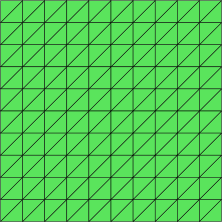
\includegraphics[width=0.4\textwidth]{../figures/struct_triangle_mesh.pdf}
    \caption{Triangular Mesh}
\end{figure}
\end{frame}

\begin{frame}
\frametitle{Linear Finite Element Method for Poisson Equation}
\begin{itemize}
\item Define local finite elements $(V_k^K, K, \mathcal{N})$, where $V_k^K :=
    \mathbb{P}_1(K)$. The degrees of freedom $\mathcal{N}$ are the values of the
    functions at the vertices:
    $$
    \mathcal{N}_i(v) = v(x_i)
    $$
\end{itemize}
\begin{figure}[htpb]
    \centering
    \includegraphics[width=0.8\textwidth]{../figures/lambda.png}
    \caption{Basis Functions}
\end{figure}
\end{frame}

\begin{frame}
\frametitle{Linear Finite Element Method for Poisson Equation}
\begin{itemize}
\item Construct the global finite element space $V_k$:
    $$
    V_k = \{v_h \in H^1(\Omega): v_h|_K \in V_k^K, \forall K \in
    \mathcal{T}_h\}.
    $$
\end{itemize}
\begin{figure}[htpb]
    \centering
    \includegraphics[width=0.6\textwidth]{../figures/femfunction_global.png}
    \caption{Global Basis Functions}
\end{figure}
\end{frame}

\begin{frame}
\frametitle{Linear Finite Element Method for Poisson Equation}
\begin{itemize}
\item Solve the finite element problem: find $u_h \in V_k$ such that
    $$
    a_h(u_h, v_h) = (f, v_h) \quad \forall v_h \in V_k,
    $$
    where
    $$
    a_h(u_h, v_h) = \sum_{K \in \mathcal{T}_h} \int_K \nabla u_h \cdot \nabla v_h \,
    \mathrm{d} x
    $$
\end{itemize}
\end{frame}

\begin{frame}
    \frametitle{Virtual Element Method for Poisson Equation}
\begin{itemize}
    \item Partition $\Omega$ into a polygonal mesh $\mathcal{T}_h$. 
\end{itemize}
\begin{figure}[htpb]
    \centering
    \includegraphics[width=0.6\textwidth]{../figures/convex.pdf}
    \caption{Polygonal Mesh}
\end{figure}
\end{frame}

\begin{frame}
    \frametitle{Virtual Element Method for Poisson Equation}
\uncover<1->{
    \begin{itemize}
        \item Define local virtual elements $(V_k^K, K, \mathcal{N})$, where 
            $$
            V_k^K := \{v \in H^1(K): v|_{\partial K} \in \mathbb{P}_1(\partial K),
            \Delta v = 0\}.
            $$ 
            The degrees of freedom $\mathcal{N}$ are the function values at the vertices.
    \end{itemize}
    \begin{figure}[htpb]
        \centering
        \includegraphics[width=0.9\textwidth]{../figures/vemlambda.png}
        \caption{Virtual Element Basis Functions}
    \end{figure}
}
\uncover<2->{
    \vspace{-5pt}
\centering{
\highlightit{Virtual element basis functions are unknown! However, the $H^1$
projection onto $\mathbb{P}_1(K)$, $\Pi_h^K$, is known.}
}}
\end{frame}

\begin{frame}
    \frametitle{Virtual Element Method for Poisson Equation}
    \begin{itemize}
        \item Construct the virtual element space $V_k$:
            $$
            V_k = \{v_h \in H^1(\Omega): v_h|_K \in V_k^K, \forall K \in
            \mathcal{T}_h\}.
            $$
    \end{itemize}
    \begin{figure}[htpb]
        \centering
        \includegraphics[width=0.6\textwidth]{../figures/vemfunction_global.png}
        \caption{Global Virtual Element Basis Functions}
    \end{figure}
\end{frame}

\begin{frame}
    \frametitle{Virtual Element Method for Poisson Equation}
    \begin{itemize}
\item Solve the virtual element problem: find $u_h \in V_k$ such that
$$
a_h(u_h, v_h) = (f, \Pi_h v_h) \quad \forall v_h \in V_k,
$$
The discrete bilinear form $a_h$ is defined as follows:
$$
a_h(u_h, v_h) = \sum_{K \in \mathcal{T}_h} a_h^K(u_h, v_h) 
$$
The local bilinear form $a_h^K$ is defined as:
$$
\begin{aligned}
a_h^K(u_h, v_h) = & \int_K \nabla \Pi_h^K u_h \cdot \nabla \Pi_h^K v_h \, \mathrm{d}
x
\uncover<2->{
\highlightit{+ S_h^K(u_h - \Pi_h^K u_h, v_h - \Pi_h^K v_h)}.
}
\end{aligned}
$$
\uncover<3->{
where $S_h^K$ is a stabilization term that must satisfy:
$$
C_* |v|_{1} \leq S_h^K(v, v) \leq C^*
|v|_{1}\quad
\forall v \in \ker{\Pi_h^K} \cap V_k^K.
$$
}
\end{itemize}
\end{frame}

\begin{frame}
    \frametitle{Advantages and Disadvantages of the VEM}
\small{
\begin{minipage}[b]{0.6\linewidth}
\textbf{Advantages:}
\begin{itemize}
    \item \textbf{Low mesh requirements:} It can be computed on arbitrary polygonal meshes.
    \item \textbf{Convenient definition of higher regularity spaces:} It allows the definition of $H^m$-conforming non-conforming spaces, with polynomial degree only needing $k \geq m$.
\end{itemize}
\vspace{10pt}
\textbf{Disadvantages:}
\begin{itemize}
    \item \textbf{Complex implementation:} Compared to finite element methods, the virtual element method is more complex to implement.
    \item \textbf{Stabilization terms:} In nonlinear problems, the choice of coefficients can have a significant impact on numerical results.
\end{itemize}
\end{minipage}
\hfill
\begin{minipage}[b]{0.38\linewidth}
    \centering
    \begin{figure}[htpb]
        \centering
        \includegraphics[width=0.65\textwidth]{../figures/four.jpg}
        \caption{Quadtree Mesh}
    \end{figure}
    \vspace{20pt}
\end{minipage}
}
\end{frame}

\section{$H^m$ conforming virtual element method in arbitrary dimension}
\begin{frame}
    \frametitle{Green's identity}
  \begin{lemma}[Green's identity]
      Let $K\in\mathbb{R}^n$, for any $v \in H^m(K)$ and $q \in H^{2m}(K)$:
      $$
      (\nabla^m v, \nabla^m q)_K = (v, (-\Delta)^m q) + \sum_{i=0}^{m-1}
      (\nabla^i v, \nabla^i(-\Delta)^{m-i-1}\partial_{\boldsymbol{\nu}}q)_{\partial K}
      $$
  \end{lemma}
  Let $\nabla_F  = \sum_{i}\boldsymbol{t}_{F, i}
  \frac{\partial v}{\partial \boldsymbol{t}_{F, i}}$, then $\nabla = \nabla_F +
  \boldsymbol{\nu}_F \frac{\partial }{\partial \boldsymbol{\nu}_F}$
  %\begin{itemize}
  %    \item $(\nabla^m v)|_F$ is continues $\Longleftrightarrow
  %        (\frac{\partial^l v}{\partial \boldsymbol{\nu}_F^l})|_F$ is continues.
  %\end{itemize}
  $$
  \begin{aligned}
  (\nabla^m v, \nabla^m q)_K
  & = (v, (-\Delta)^m q)_K + \sum_{i=0}^{m-1}
     \sum_{l=0}^i\sum_{F\in\mathcal{F}^1(K)}
     \left(\frac{i!}{l!(i-l!)}\right)^2
     \\
     & \quad\quad\quad\quad\quad(\nabla^{l}_{F}\partial^{i-l}_{\boldsymbol\nu_F} v,
     \nabla^{l}_{F}
     (-\Delta)^{m-i-1}\partial^{i-l+1}_{\boldsymbol\nu_F}q)_F\\
  \end{aligned}
  $$
\end{frame}

\begin{frame}
    \frametitle{$H^m$ conforming function}
  If $v \in H^m(K_1)$ and $v \in H^m(K_2)$, then:\\
  \vspace{0.5cm}
  \centering
  $v \in H^m(K_1\cap K_2) \Longleftrightarrow  
  (\frac{\partial^l v}{\partial \boldsymbol{\nu}_F^l})|_F$ is continues.

  \begin{figure}[H]
    \centering
    \includegraphics[scale=0.2]{../figures/dodecahedron.pdf}
  \end{figure} 
\end{frame}


\begin{frame}
\frametitle{$H^m$-Conforming virtual element in $\mathbb{R}^1$}
Let $K$ is an interval, \bf{DoFs}:
\begin{itemize}
    \item $h_K^j v^{(j)}(\delta) \quad \forall \delta \in \mathcal{F}^1(K),
        j = 0, 1, \dots, m-1$,
    \item $\frac{1}{|K|}(v, q)_K \quad \forall q \in \mathbb{P}_{k-2m}(K)$. 
\end{itemize}
\bf{shape function space}:
$$
V_k^m(K) := \{v \in H^m(K): v^{(2m)}\in\mathbb{P}_{k-2m}(K)\} = 
\left\{ 
\begin{aligned}
    \mathbb{P}_{k} \quad & k\geq 2m-1\\
    \mathbb{P}_{2m-1} \quad & k < 2m-1
\end{aligned}
\right.
$$
\end{frame}

\begin{frame}
\frametitle{$H^m$-Conforming virtual element in $\mathbb{R}^2$}
Let $K$ is a polygon, define a preliminary space:
$$
\small{
\begin{aligned}
  \widetilde{V}_k^m(K) := \Big\{v \in H^m(K) : & (-\Delta)^m v \in P_k(K),\\ 
      & \frac{\partial^j v}{\partial \boldsymbol{\nu}_e^j} \in V_{k-j}^{m-j}(e) \quad 
    \forall e \in \mathcal{F}^1(K), j=0, 1, \dots, m-1\Big\}.
\end{aligned}
}
$$
\begin{itemize}
    \item $\mathbb{P}_k(K) \subseteq \widetilde{V}_k^m(K)$ but 
        $\mathbb{P}_{k+1}(K) \not\subseteq \widetilde{V}_k^m(K)$.
    \item $\nabla^j v$ is continuous on $\partial K$.
\end{itemize}

\bf{Choose DoFs as}:
\begin{itemize}
    \item $h_K^j \nabla^{j}v(\delta) \quad \forall \delta \in \mathcal{F}^2(K),
        j = 0, 1, \dots, m-1$,
    \item $\frac{h_K^j}{|e|}(\frac{\partial^j v}{\partial \boldsymbol{\nu}_e^j}, q) \quad 
        \forall q \in \mathbb{P}_{k-2m+j}(e), e \in \mathcal{F}^1(K), 
        j = 0, 1, \dots, m-1$,
    \item $\frac{1}{|K|}(v, q)_K \quad \forall q \in \mathbb{P}_{k-2m}(K)$. 
\end{itemize}
\end{frame}

\begin{frame}
\frametitle{$H^m$-Conforming virtual element in $\mathbb{R}^2$}
    \textbf{shape function space as}:
    $$
    V_k^m(K) := \{v \in \widetilde{V}_k^m(K): (v, q) = (\Pi_k^Kv, q) \quad 
        \forall q \in \mathbb{P}_{k-2m}^{\perp}(K)\}
    $$
    where $\Pi_k^K : \widetilde{V}_k^m(K) \to \mathbb{P}_k(K)$ defined as:
    $$
    \begin{aligned}
        (\nabla^m \Pi_k^K v, \nabla^m q) &  = (\nabla^m v, \nabla^m q) \quad
        \forall q \in \mathbb{P}_k(K)\\
        \sum_{\delta\in\mathcal{F}^2(K)}(\nabla^j\Pi_k^K v)(\delta) & = 
        \sum_{\delta\in\mathcal{F}^2(K)}(\nabla^j v)(\delta) \quad j = 0, 1,
        \dots, m-1.
    \end{aligned}
    $$
    Let $Q_k^K : \widetilde{V}_k^m(K) \to \mathbb{P}_k(K)$ is $L^2$ projection
    then:
    $$
    Q_k^K = \Pi_k^K + Q_{k-2m} - Q_{k-2m}\Pi_k^K 
    $$
\end{frame}
\begin{frame}
    \frametitle{$H^m$-Conforming virtual element in $\mathbb{R}^n$}
    \begin{figure}[H]
        \centering
        \includegraphics[scale=0.3]{../figures/bitmap.pdf}
    \end{figure}
\end{frame}

\begin{frame}
    \frametitle{$H^m$-Conforming virtual element in $\mathbb{R}^n$}
    Let $K \subset \mathbb{R}^n$ is a polytope, define a preliminary space:
    $$
    \small{
    \begin{aligned}
      \widetilde{V}_k^m(K) := \Big\{v \in  H^m(K) :&  (-\Delta)^m v \in P_k(K),\\
          & \nabla^j v|_{\mathcal{S}^r(K)} \in H^1(\mathcal{S}^r(K),\mathbb{S}_n(j)), \\
          & \qquad\qquad j = 0, 1, \dots, m-1, r = 1, 2, \dots, n\\
          & \frac{\partial^j v}{\partial
          \boldsymbol{\nu}_F^{\boldsymbol{\alpha}}} \in V_{k-j}^{m-j}(F) \quad 
          \forall F \in \mathcal{F}^r(K), \\
          &\qquad\qquad r = 1, 2, \dots, n-1, \boldsymbol{\alpha} \in \mathcal{A}_{m-1}^r.
          \Big\}
    \end{aligned}
    }
    $$
    \begin{itemize}
        \item $\mathbb{P}_k(K) \subseteq \widetilde{V}_k^m(K)$ but 
            $\mathbb{P}_{k+1}(K) \not\subseteq \widetilde{V}_k^m(K)$.
    \end{itemize}
\end{frame}
\begin{frame}
    \frametitle{$H^m$-Conforming virtual element in $\mathbb{R}^n$}
    \textbf{Choose DoFs as} $\mathcal{N}_k^m(K)$:
  \begin{itemize}
    \item $h_K^j\nabla^{j}v(\delta) \quad\forall~\delta\in\mathcal F^{n}(K),\;
         j=0,1,\cdots,m-1,$
    \item $\frac{h_K^{j}}{|F|}(
        \frac{\partial^{\boldsymbol{\alpha}}v}{\partial
    \boldsymbol{\nu}_F^{\boldsymbol{\alpha}}}, q)_F
        \quad\forall~q\in\mathbb P_{k-2m+j}(F), F\in\mathcal
        F^{r}(K),$\\
        $\quad\quad\quad\quad\quad\quad
        \boldsymbol{\alpha}\in \mathcal{A}_j^r, 
        r = 1, 2, \dots, n-1, j=0,1,\cdots,m-1$
    \item $\frac{1}{|K|}(v, q)_K \quad\forall~q\in\mathbb P_{k-2m}(K)$ 
  \end{itemize}
  \textbf{shape function space as}:
    $$
    V_k^m(K) := \{v \in \widetilde{V}_k^m(K): (v, q) = (\Pi_k^Kv, q) \quad 
        \forall q \in \mathbb{P}_{k-2m}^{\perp}(K)\}
    $$
where $\Pi_k^K : \widetilde{V}_k^m(K) \to \mathbb{P}_k(K)$ defined as:
$$
\begin{aligned}
    (\nabla^m \Pi_k^K v, \nabla^m q) &  = (\nabla^m v, \nabla^m q) \quad
    \forall q \in \mathbb{P}_k(K)\\
    \sum_{\delta\in\mathcal{F}^2(K)}(\nabla^j\Pi_k^K v)(\delta) & = 
    \sum_{\delta\in\mathcal{F}^2(K)}(\nabla^j v)(\delta) \quad j = 0, 1,
    \dots, m-1.
\end{aligned} 
$$
\end{frame}

\begin{frame}
    \frametitle{VEM VS FEM}
\begin{minipage}[b]{0.49\linewidth}
    \large{\textbf{FEM}}:
    \begin{itemize}
        \item Include super-smooth DoFs.
        \item Requires a polynomial degree of at least $2^n \times (m-1)
            +1$.
    \end{itemize}
    \vspace{22pt}
\end{minipage}
\hfill
\begin{minipage}[b]{0.49\linewidth}
    \large{\textbf{VEM}}:
    \begin{itemize}
        \item Does not include super-smooth DoFs.
        \item Require a polynomial degree only greater than $m$
    \end{itemize}
    \vspace{10pt}
\end{minipage}
\begin{minipage}[b]{0.49\linewidth}
    \begin{figure}[htpb]
        \centering
        \includegraphics[width=0.5\textwidth]{../figures/hmvem/smooth3d.pdf}
        \caption{The DoFs of $H^2$-conforming FEM}
    \end{figure}
\end{minipage}
\hfill
\begin{minipage}[b]{0.49\linewidth}
    \begin{figure}[htpb]
        \centering
        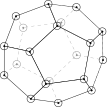
\includegraphics[width=0.5\textwidth]{../figures/hmvem/hmdof3d.pdf}
        \caption{The DoFs of $H^2$-conforming VEM}
    \end{figure}
\end{minipage}
\end{frame}

\begin{frame}
\frametitle{Polyharmonic equation}

\begin{definition}[Polyharmonic equation]
  Let $\Omega = (0, 1)\times(0, 1)$, Consider polyharmoic equation:
  $$
  \left\{
  \begin{aligned}
      (-\Delta)^m u + c u & = f \quad \Omega\\
      \frac{\partial^j u}{\partial \boldsymbol{\nu}^j} & = 0 \quad \partial\Omega,
      j = 0, 1, \dots, m-1.
  \end{aligned}
  \right.
  $$
\end{definition}
\begin{definition}[Variational form]
Find $u\in H_0^m(\Omega)$ such that
$$
(\nabla^mu, \nabla^mv)+c(u, v)=(f, v)\quad\forall~v\in H_0^m(\Omega),
$$
where $f\in L^2(\Omega)$ and constant $c\geq0$.
\end{definition}
\hspace*{\fill} \\
\hspace*{\fill} \\
\hspace*{\fill} \\
\hspace*{\fill} \\
\hspace*{\fill} \\
\end{frame}

\note[itemize]{
\item 
    \begin{CJK}{UTF8}{gkai}
        $H^m$ 协调元的一个直接应用就是多重调和方程,
        我们考虑这样一个带有低阶项的多重调和方程, 他的变分形式就是下面这样.
    \end{CJK}
\item A direct application of $H^m$ conforming elements is in the context of
    polyharmonic equations. Consider a polyharmonic equation with lower-order
    terms, this is its variational form.
}

\begin{frame}
\begin{definition}[VEM for polyharmonic equation]
  Let $\mathcal{T}_h$ is a polytope mesh on $\Omega$, 
  define the virtual element space:
  $$
  V_h:=\{v_h\in H_0^m(\Omega): v_h|_K\in V_{k}^{m}(K) \textrm{ for each } K\in\mathcal T_h\}.
  $$
  The VEM of polyharmonic equation is that: {\bf find $u_h \in V_h$ statify}: 
  $$
  a_{h}(u_h, v_h)=\langle f, v_h\rangle\quad\forall~v_h\in V_h,
  $$
  {\bf where} $\langle f, v_h\rangle:=\sum\limits_{K\in\mathcal T_h}(f,
  Q_k^Kv_h)_K, a_h(u_h, v_h):=\sum_{K\in\mathcal T_h}a_{h,K}(u_h, v_h),$
  $$
  \begin{aligned}
  a_{h,K}(u_h, v_h):=&\,(\nabla^m\Pi_k^Ku_h,
  \nabla^m\Pi_k^Kv_h)_K+S_K(u_h-\Pi_k^Ku_h,v_h-\Pi_k^Kv_h) \\
  &+c(Q_k^Ku_h, Q_k^Kv_h)_K.
  \end{aligned}
  $$
\end{definition}
\hspace*{\fill} \\
\hspace*{\fill} \\
\hspace*{\fill} \\
\end{frame}

\begin{frame}
  \frametitle{Stablized term}
  \begin{definition}[Stablized term]
    \footnotesize{
    $$
    S_K(w,v):=\sum_{r=1}^{n}\sum_{F\in\mathcal F^{r}(K)}\sum_{\alpha\in A_{r}\atop
    |\alpha|\leq
    m-1}h_K^{r+2|\alpha|-2m}\bigg(Q_{k-2m+|\alpha|}^{F}\frac{\partial^{|\alpha|}w}{\partial
    \boldsymbol{\nu}_{F}^{\alpha}},Q_{k-2m+|\alpha|}^{F}\frac{\partial^{|\alpha|}v}{\partial
    \boldsymbol{\nu}_{F}^{\alpha}}\bigg)_{F}
    $$
  }
  \end{definition}
  \begin{lemma}
      $$
      S_K(v-\Pi_k^Kv,v-\Pi_k^Kv)\eqsim |v-\Pi_k^Kv|_{m,K}^2\quad\forall~v\in V_{k}^{m}(K).
      $$
  \end{lemma}
    \begin{lemma}
    $$
    a_{h,K}(w, v)\lesssim (|w|_{m,K}+\|w\|_{0,K})(|v|_{m,K}+\|v\|_{0,K})\quad\forall~w,v\in V_{k}^{m}(K),
    $$
    $$
    a_{h}(v_h, v_h)\eqsim |v_h|_{m}^2\quad\forall~v_h\in V_h.   
    $$
    \end{lemma}
\end{frame}


\begin{frame}
\frametitle{Error estimate}
\begin{theorem}\label{errorestimate}
Let $u\in H^s(\Omega)\cap H_0^m(\Omega)$ with $s\geq m$ be the solution of the
polyharmonic equation, and $u_h\in V_h$ be the solution
of the conforming virtual element method. Assume the mesh. Assume
$f\in H^m(\mathcal T_h)$. Then we have
$$
|u-u_h|_m\lesssim h^{\min\{s,k+1\}-m}|u|_{\min\{s,k+1\}}+\textrm{osc}_h(f),
$$
$$
|u-\Pi_hu_h|_{m,h}\lesssim h^{\min\{s,k+1\}-m}|u|_{\min\{s,k+1\}}+\textrm{osc}_h(f),
$$
where $\textrm{osc}_h^2(f):=\sum\limits_{K\in\mathcal T_h}h_K^{2m}\|f-Q_k^Kf\|_{0,K}^2$.
\end{theorem}

\end{frame}

\begin{frame}
  \frametitle{Biharmonic equation}
  Let $\Omega = (0, 1)\times(0, 1)$, Consider biharmoic equation:
  $$
  \left\{
  \begin{aligned} 
      \Delta^2 u + 2u & = f \quad \Omega\\
      \frac{\partial^j u}{\partial \boldsymbol{n}^j} & = 0 \quad \partial\Omega,
      j = 0, 1.
  \end{aligned}
  \right.
  $$
  with true solution $u = \sin^2(\pi x)\sin^2(\pi y)$.

\begin{figure}[htb p]
\centering
\begin{minipage}[t]{0.49\linewidth}
\centering
\includegraphics[width=4cm]{../figures/convex.pdf}
\captionsetup{font={small}}
\caption{Convex polygon mesh $\mathcal T_0$}
\end{minipage}%
\begin{minipage}[t]{0.49\linewidth}
\centering
\includegraphics[width=4cm]{../figures/nonconvex.pdf}
\captionsetup{font={small}}
\caption{Non-convex polygon mesh $\mathcal T_1$}
\end{minipage}%
\centering
%\caption{\small Convex polygon mesh $\mathcal T_0$(left) and non-convex polygon mesh 
%$\mathcal T_1$(right).}
\end{figure}
\end{frame}

\begin{frame}
  \frametitle{Numberical result of VEM}
\begin{figure}[htbp]
\centering
\begin{minipage}[t]{0.49\linewidth}
\centering
\includegraphics[width=5cm]{../figures/H2_convex.pdf}
%\caption{Numberical result of example with $\mathcal T_0$.}
\end{minipage}%
\begin{minipage}[t]{0.49\linewidth}
\centering
\includegraphics[width=5cm]{../figures/H2_nonconvex.pdf}
%\caption{[Numberical result of example with $\mathcal T_1$].}
\end{minipage}%
\centering
\caption{Error $|u - \Pi_h u_h|_{2, h}$ of biharmonic 
    equation with $m=2$ on convex polygon mesh $\mathcal T_0$(left) 
and non-convex polygon mesh $\mathcal T_1$(right) with $k = 2, 3, 4, 5$.}
\label{fig:H2error}
\end{figure} 
\end{frame}

\begin{frame}
  \frametitle{Triharmonic equation}
  Let $\Omega = (0, 1)\times(0, 1)$, Consider triharmoic equation:
  $$
  \left\{
  \begin{aligned}
      -\Delta^3 u + 2u & = f \quad \Omega\\
      \frac{\partial^j u}{\partial \boldsymbol{n}^j} & = 0 \quad \partial\Omega,
      j = 0, 1, 2.
  \end{aligned}
  \right.
  $$
  with true solution $u = \sin^3(\pi x)\sin^3(\pi y)$.

\begin{figure}[htbp]
\centering
\begin{minipage}[t]{0.49\linewidth}
\centering
\includegraphics[width=4cm]{../figures/convex.pdf}
\captionsetup{font={small}}
\caption{Convex polygon mesh $\mathcal T_0$}
\end{minipage}%
\begin{minipage}[t]{0.49\linewidth}
\centering
\includegraphics[width=4cm]{../figures/nonconvex.pdf}
\captionsetup{font={small}}
\caption{Non-convex polygon mesh $\mathcal T_1$}
\end{minipage}%
\centering
%\caption{\small Convex polygon mesh $\mathcal T_0$(left) and non-convex polygon mesh 
%$\mathcal T_1$(right).}
\end{figure}

\end{frame}

\begin{frame}
  \frametitle{Numberical result of VEM}
\begin{figure}[htbp]
\centering
\begin{minipage}[t]{0.49\linewidth}
\centering
\includegraphics[width=5cm]{../figures/H3_convex.pdf}
%\caption{Numberical result of example with $\mathcal T_0$.}
\end{minipage}%
\begin{minipage}[t]{0.49\linewidth}
\centering
\includegraphics[width=5cm]{../figures/H3_nonconvex.pdf}
%\caption{[Numberical result of example with $\mathcal T_1$].}
\end{minipage}%
\centering
\caption{Error $|u - \Pi_h u_h|_{3, h}$ of 
    triharmonic equation with $m=3$ on convex polygon mesh $\mathcal T_0$(left) 
and non-convex polygon mesh $\mathcal T_1$(right) with $k = 3, 4, 5, 6$.}
\label{fig:H3error}
\end{figure}
\end{frame}
\section{Stabilization-free virtual element method}
\begin{frame}
\frametitle{Virtual Element Method For Poisson Equation}
Given the virtual element space $V_h$, the virtual element method for the
Poisson equation is to find $u_h \in V_h$ such that
$$
a_h(u_h, v_h) = (f, v_h) \quad \forall v_h \in V_h,
$$
where the discrete bilinear form $a_h$ is defined as:
$$
a_h(u_h, v_h) = \sum_{K \in \mathcal{T}_h} a_h^K(u_h, v_h)
$$
$$
a_h^K(u_h, v_h) = \int_K \nabla \Pi_h^K u_h \cdot \nabla \Pi_h^K v_h \, \mathrm{d}x + \highlightit{S_h^K(u_h - \Pi_h^K u_h, v_h - \Pi_h^K v_h)}.
$$
The stabilizer term $S_h^K$ needs to satisfy:
$$
c_* |v|_{1, K}^2 \leq S_h^K(v, v) \leq C_* |v|_{1, K}^2 \quad \forall v \in 
V_h^K \cap \mathrm{ker}(\Pi_h^K).
$$
\end{frame}

\begin{frame}
\frametitle{Stabilization-free Virtual Element Method}

\begin{minipage}[b]{0.6\linewidth}
\uncover<1->{
\small{
\textbf{Objective}: Find an appropriate space $W_h^K$ such that
\begin{itemize}
    \item The projection $Q^K $ from $ \nabla V_h^K$ onto $ W_h^K $ can be computed.
    \item $ \|Q^K \nabla v\| \eqsim \|\nabla v\| \quad \forall v \in V_h^K $.
\end{itemize}
\vspace{10pt}
}
\uncover<2->{
\textbf{Method:}
Divide the polyhedron $ K $ into a simplicial mesh $ \mathcal{T}_K $,
and on $ \mathcal{T}_K $, construct the $ k $-BDM element space $ \tilde{W}_h^k
$, and define $ W_h^{k}$ as
$$
W_h^{k-1} = \{\boldsymbol{v} \in \tilde{W}_h^{k-1}: \mathrm{div} \boldsymbol{v} \in
\mathbb{P}_{k-2}(K)\}.
$$
Then, the $ L^2 $ orthogonal projection $ Q^K $ from $ \nabla V_h^K $ onto 
$W_h^K$ can be computed as:
$$
\begin{aligned}
(Q^K \nabla\boldsymbol{v}, \boldsymbol{w})_K & = (\nabla v, \boldsymbol{w})_K\\
& = (v, \mathrm{div} \boldsymbol{w})_K + \langle v, \boldsymbol{w} \cdot 
\boldsymbol{n}\rangle_{\partial K}.
\end{aligned}
$$
}
}
\end{minipage}
\hfill
\begin{minipage}[b]{0.36\linewidth}
    \centering
    \uncover<2->
{
    \begin{figure}[htpb]
        \centering
        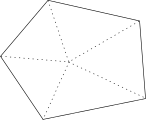
\includegraphics[width=0.75\textwidth]{../figures/splite_polygon.pdf}
        \caption{Splitting polygon $ K $ into triangles.}
    \end{figure}
}
\vspace{45pt}
\end{minipage}
\end{frame}

\begin{frame}
  \frametitle{Mesh Conditions}
  The mesh $\mathcal{T}_h$ is required to satisfy the following conditions:
  \begin{itemize}
    \item For any element $K \in \mathcal{T}_h$ and face $F \in \mathcal{F}_h^r$,
        where $1 \leq r \leq d-1$, the element is star-shaped with respect to a ball of radius $\rho_K$, and
        $\rho_K / h_K$ has a lower bound.
    \item For any element $K \in \mathcal{T}_h$, there exists an quasi-uniform simplicial mesh
        $\mathcal{T}_K$ that partitions $K$, and the union $\cup_{K \in \mathcal{T}_h} \mathcal{T}_K$
        forms a shape-regular simplicial mesh.
  \end{itemize}
  \vspace{10pt}
\begin{minipage}[b]{0.49\linewidth}
    \begin{figure}[htpb]
      \centering
      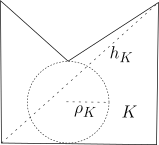
\includegraphics[width=0.55\textwidth]{../figures/star-shaped.pdf}
      \caption{Star-shaped}
    \end{figure}
\end{minipage}
\hfill
\begin{minipage}[b]{0.49\linewidth}
    \centering
    \begin{figure}[htpb]
        \centering
        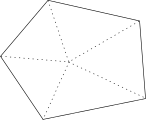
\includegraphics[width=0.55\textwidth]{../figures/splite_polygon.pdf}
        \caption{quasi-uniform simplicial mesh}
    \end{figure}
\end{minipage}

\end{frame}

\begin{frame}
    \frametitle{Finite Element Differential $d-2$ Form}
For $T \in \mathcal{T}_K$, with $\mathbb{P}_k(T, \mathbb{K})$ as the shape function space, the following degrees of freedom are defined:
$$
\begin{aligned}
((\bsn_{1}^{e})^{\mathsf{T}}\tau\bsn_{2}^{e},q)_{e}, & \quad q\in\mathbb{P}_{k}(e), e\in\mathcal{E}(T), \\
(\mathrm{div}_{F}(\tau\bsn),q)_{F}, & \quad q\in\mathbb{P}_{k-1}(F)/\mathbb{R}, F\in\mathcal{F}(T), \\
(\tau\bsn,\bsq)_F, & \quad q\in\mathbb{P}_{k-2}(F;\mathbb{K})\bsx, F\in\mathcal{F}(T), \\
(\operatorname{div}\tau,q)_{T}, & \quad q\in\mathbb{P}_{k-3}(T;\mathbb{K})\bsx, \\
(\tau,q)_{T}, & \quad \bsq\in\mathbb{P}_{k-2}(T;\mathbb{K})\cap\ker(\bsx).
\end{aligned}
$$
Define the $d-2$ form space $V^{d-2}_k$:
$$
\begin{aligned}
V^{d-2}_k = \{\tau \in L^2(K; \mathbb{K}) : & \tau|_T \in \mathbb{P}_k(T, \mathbb{K}), \forall T \in \mathcal{T}_K, \\
& \text{first three conditions are single-valued}\}.
\end{aligned}
$$
\uncover<2->{
\small{
\highlightit{
When $d = 2$, $V^{d-2}_k$ is the Lagrange element space.
When $d = 3$, $V^{d-2}_k$ is the Nédélec element space.
}
}
}
\end{frame}

\begin{frame}
    \frametitle{$H(\diver)$-conforming Finite Element Space: BDM Elements}
For $k \geq 2$, define the $H(\mathrm{div})$ BDM element space $V^{BDM}_{k-1}$:
$$
V^{BDM}_{k-1}(K) := \{\bsv \in H(\diver, K) : \bsv|_T \in
\mathbb{P}_{k-1}(T; \mathbb{R}^d), \forall T \in \mathcal{T}_K\}.
$$
The local degrees of freedom of the BDM element on the simplex $T$ are:
$$
\begin{aligned}
(v\cdot\bsn,q)_{F}, & \quad
q\in\mathbb{P}_{k-1}(F), F\in\mathcal{F}(T), \\
(\diver v, q)_{T}, & \quad q\in\mathbb{P}_{k-2}(T)/\mathbb{R}, \\
(v, \bsq)_T, & \quad
\bsq\in\mathbb{P}_{k-3}(T;\mathbb{K})\bsx.
\end{aligned}
$$
Define the trace-zero subspace of $V^{BDM}_{k-1}$:
$$
\mathring{V}_{k-1}^{\mathrm{BDM}}(K):=V_{k-1}^{\mathrm{BDM}}(K)\cap\bsH_{0}(\mathrm{div},K).
$$
\end{frame}

\begin{frame}
    \frametitle{$H(\mathrm{div})$-conforming Finite Element Space: RT Elements}
For the case $k=1$, define the lowest-order RT element space $V^{RT}$:
$$
V^{RT}(K) := \{\bsv \in H(\diver, K) : \bsv|_T \in
\mathbb{P}_{0}(T; \mathbb{R}^d) + \bsx\mathbb{P}_{0}(T),
\forall T \in \mathcal{T}_K\}.
$$
The local degrees of freedom of the RT element on the simplex $T$ are:
$$
(v\cdot\bsn,q)_{F}, \quad
q\in\mathbb{P}_{0}(F), F\in\mathcal{F}(T)
$$
Define its trace-zero subspace:
$$
\mathring{V}^{\mathrm{RT}}(K):=V^{\mathrm{RT}}(K)\cap\bsH_{0}(\mathrm{div},K).
$$
\end{frame}

\begin{frame}
    \frametitle{Finite Element Complex}
For the case $k \geq 2$, the following finite element complex is exact:
$$
\begin{aligned}
V_{k}^{d-2}(K) & \xrightarrow{\mathrm{div~skw}}
V_{k-1}^{\mathrm{BDM}}(K) \xrightarrow{\mathrm{div}} V_{k-2}^{L^{2}}(K)
\to 0, \\
V_{1}^{d-2}(K) & \xrightarrow{\mathrm{div~skw}}
V^{\mathrm{RT}}(K) \xrightarrow{\mathrm{div}} V_{0}^{L^{2}}(K)
\to 0, \\
\mathring{V}_{k}^{d-2}(K) & \xrightarrow{\mathrm{div~skw}}
\mathring{V}_{k-1}^{\mathrm{BDM}}(K) \xrightarrow{\mathrm{div}}
\mathring{V}_{k-2}^{L^{2}}(K) \to 0, \\
\mathring{V}_{1}^{d-2}(K) & \xrightarrow{\mathrm{div~skw}}
\mathring{V}^{\mathrm{RT}}(K) \xrightarrow{\mathrm{div}}
\mathring{V}_{0}^{L^{2}}(K) \to 0,
\end{aligned}
$$
where $\mathring{V}_{k-2}^{L^{2}}(K) = V_{k-2}^{L^{2}}(K) / \mathbb{R}$.
$$
V_{k-2}^{L^{2}}(K) = \{\tau \in L^2(K; \mathbb{K}) : \tau|_T \in
\mathbb{P}_{k-2}(T), \forall T \in \mathcal{T}_K\}.
$$
\end{frame}

\begin{frame}
    \frametitle{$H(\mathrm{div})$-conforming Macro-element Space $V^{\mathrm{div}}_{k-1}$}
Define the $H(\mathrm{div})$-conforming macro-element space $V^{\mathrm{div}}_{k-1}(K)$:
$$
V^{\mathrm{div}}_{k-1}(K) := \{\bsv \in V^{BDM}_{k-1}(K) : \diver
\bsv \in \mathbb{P}_{k-2}(K)\}.
$$
For the case $k=1$, define:
$$
V^{\mathrm{div}}_{0}(K) := \{\bsv \in V^{RT}(K) : \diver
\bsv \in \mathbb{P}_{0}(K)\}.
$$
The following complex is exact:
$$
\begin{aligned}
V_{k}^{d-2}(K) & \xrightarrow{\mathrm{div~skw}}
V^{\mathrm{div}}_{k-1}(K) \xrightarrow{\mathrm{div}}
\mathbb{P}_{\max\{k-2, 0\}}(K) \to 0
\end{aligned}
$$
According to the finite element complex, we can decompose $V^{\mathrm{div}}_{k-1}(K)$ as:
$$
V^{\mathrm{div}}_{k-1}(K) = \mathrm{div~skw}V_{k}^{d-2}(K) \oplus 
(\boldsymbol{x-x}_K)\mathbb{P}_{\max\{k-2, 0\}}(K).
$$
\end{frame}

\begin{frame}
    \frametitle{$H(\mathrm{div})$ Conforming Macro-element Space $\mathbb{V}^{\mathrm{div}}_{k-1}$}
    $V^{\mathrm{div}}_{k-1}$ is not polynomial on the boundary of $K$, so we take its subspace 
    $\mathbb{V}^{\mathrm{div}}_{k-1}$:
    $$
    \mathbb{V}^{\mathrm{div}}_{k-1}(K) := \{\bsv \in
        V^{\mathrm{div}}_{k-1}(K) :
        \bsv \cdot \bsn|_F \in \mathbb{P}_{k-1}(F),
    \forall F \in \mathcal{F}(K)\}.
    $$
    Its degrees of freedom are:
    $$
    \begin{aligned}
        (v\cdot\bsn,q)_{F}, & \quad
        q \in \mathbb{P}_{k-1}(F), F \in \mathcal{F}(K), \\
        (\diver v, q)_{K}, & \quad q \in \mathbb{P}_{\max\{k-2, 0\}}(K)/\mathbb{R}, \\
        (v, \bsq)_K, & \quad
        \bsq \in \diver \mathring{V}_k^{d-2}(K).
    \end{aligned}
    $$
    Functions in $\mathbb{V}_{k-1}^{\mathrm{div}}$ satisfy the following norm equivalence:
    $$
    \|\bsv\|_{0, K} \eqsim h_K\|\diver \bsv\|_{0, K} + 
    \sup_{\psi \in \diver \mathring{V}_k^{d-2}(K)}\frac{(\bsv,
    \psi)_K}{\|\psi\|_{0, K}} + \sum_{F \in \mathcal{F}(K)}h_F^{1/2}\|v\cdot
    \bsn\|_{0, F}.
    $$
\end{frame}

\begin{frame}
\frametitle{Nonconforming VEM: Space}
Define the non-conforming virtual element space:
$$
\begin{aligned}
    V_k(K) := \{v \in H^1(K): & \partial_n v|_{F} \in \mathbb{P}_{k-1}(F), 
        \forall F \in \mathcal{F}(K), \\
    & \Delta v \in \mathbb{P}_{k}(K),\\
    & (v-\Pi_k^K v, q)_K = 0 \quad \forall q \in
    \mathbb{P}_{k-2}^{\perp}(K)\}.
\end{aligned}
$$
where $\Pi_k^K$ is the $H^1$ projection onto $\mathbb{P}_k(K)$.
The degrees of freedom for virtual elements are:
$$
\begin{aligned}
    \frac{1}{|F|}(v, q)_{F}, & \quad q \in \mathcal{M}_{k-1}(F), \\
    \frac{1}{|K|}(v, q)_{K}, & \quad q \in \mathcal{M}_{k-2}(K), \\
\end{aligned}
$$
where $\mathcal{M}_{k-1}(F)$ and $\mathcal{M}_{k-2}(K)$ are the scaled monomials on $F$ and $K$, respectively.
Define $Q_{K, k-1}^{\mathrm{div}}$ as the $L^2$ projection of $\nabla V_k(K)$ onto
$\mathbb{V}^{\mathrm{div}}_{k-1}(K)$:
$$
(Q_{K, k-1}^{\mathrm{div}}\nabla v, \bsw)_K := (\nabla v,
\bsw)_K = -(v, \diver \bsw)_K + \langle v, \bsw 
\cdot \bsn\rangle_{\partial K}.
$$
\end{frame}

\begin{frame}
    \frametitle{Non-conforming Virtual Element Method: Norm Equivalence}
    \begin{lemma}
        The following Inf-Sup condition holds:
        $$
        \|\nabla v\| \leq C \sup_{\bsw \in
        \mathbb{V}^{\mathrm{div}}_{k-1}(K)}\frac{(\nabla v,
        \bsw)_K}{\|\bsw\|} \quad \forall v \in V_k(K).
        $$
        where $C$ is independent of the mesh size and depends on the polynomial degree $k$, the spatial dimension $d$, the star-shaped parameter of the polytope, and the quasi-uniformity and shape-regularity parameters of the mesh.
        
        The following norm equivalence holds:
        $$
        \|Q_{K, k-1}^{\mathrm{div}}\nabla v\|_{0, K} \eqsim \|\nabla v\|_{0, K} 
        \quad \forall v \in V_k(K).
        $$
    \end{lemma}
\end{frame}

\begin{frame}
\frametitle{Non-conforming VEM for the Poisson Equation}
\small{
The unstable virtual element method is defined as: find $u_h \in V_k$ such that
$$
a_h(u_h, v_h) = (f, Q_h v_h) \quad \forall v_h \in V_k,
$$
where $a_h$ is defined as:
$$
a_h(u_h, v_h) = \sum_{K \in \mathcal{T}_h} a_h^K(u_h, v_h),
$$
$$
a_h^K(u_h, v_h) = (Q_{K, k-1}^{\mathrm{div}}\nabla u_h, Q_{K,
k-1}^{\mathrm{div}}\nabla v_h)_K.
$$
The element-wise discrete bilinear form 
$a_h^K$ satisfies the following stability condition:
$$
c_* |v|_{1, K}^2 \leq a_h^K(v, v) \leq C_* |v|_{1, K}^2 \quad \forall v \in
V_k^K.
$$
\begin{theorem}
Assume $u \in H^{k+1}(\Omega), f \in H^{k-1}(\Omega)$, then the above virtual element method
is stable, and we have:
$$
|u - u_h|_{1, \Omega} \leq C h^{k}
(|u|_{k+1, \Omega} + |f|_{k-1, \Omega}).
$$
\end{theorem}
}
\end{frame}

\begin{frame}
\frametitle{Conforming Virtual Element Method: Space}
Assume that all faces of the polyhedron are simplicial. Define the $H^1$ conforming virtual element space:
$$
\begin{aligned}
    V_k(K) := \{v \in H^1(K): & v|_{\partial K} \in H^1(\partial K), v|_F \in 
        \mathbb{P}_k(e), \forall e \in \mathcal{F}(K),
    \Delta v \in \mathbb{P}_{k}(K),\\
    & (v-\Pi_k^K v, q)_K = 0 \quad \forall q \in
    \mathbb{P}_{k-2}^{\perp}(K)\}.
\end{aligned}
$$
where $\Pi_k^K$ is the $H^1$ projection onto $\mathbb{P}_k(K)$. 
The virtual element degrees of freedom are:
$$
\begin{aligned} 
    v(\delta), & \quad \delta \in \mathcal{\Delta}_0(K), \\
    \frac{1}{|e|}(v, q)_{e}, & \quad q \in \mathcal{M}_{k-j-1}(e), \forall e \in
    \Delta_j(K), j = 1, \dots, d-1,\\
    \frac{1}{|K|}(v, q)_{K}, & \quad q\in \mathcal{M}_{k-2}(K), \\
\end{aligned}
$$
where $\mathcal{M}_{k-j-1}(e)$ and $\mathcal{M}_{k-2}(K)$ are the scaling monomials on $e$ and $K$, respectively. 
Define $Q_{K, k-1}^{\mathrm{div}}$ as the $L^2$ projection of $\nabla V_k(K)$ onto
$\mathbb{V}^{\mathrm{div}}_{k}(K)$:
$$
(Q_{K, k}^{\mathrm{div}}\nabla v, \bsw)_K := (\nabla v,
\bsw)_K = -(v, \diver \bsw)_K + \langle v, \bsw 
\cdot \bsn\rangle_{\partial K}.
$$
\end{frame}

\begin{frame}
    \frametitle{Conforming Virtual Element Method: Norm Equivalence}
    \begin{lemma}
        The following Inf-Sup condition holds:
        $$
        \|\nabla v\| \leq C \sup_{\bsw \in
        \mathbb{V}^{\mathrm{div}}_{k}(K)}\frac{(\nabla v,
        w)_K}{\|\bsw\|} \quad \forall v \in V_k(K).
        $$
        where $C$ depends on the mesh size, polynomial degree $k$, spatial dimension $d$, the star-shape parameter of the polyhedron, as well as the quasi-uniformity and shape regularity parameters of the mesh.
        
        The following norm equivalence holds:
        $$
        \|Q_{K, k}^{\mathrm{div}}\nabla v\|_{0, K} \eqsim \|\nabla v\|_{0, K} 
        \quad \forall v \in V_k(K).
        $$
    \end{lemma}
\end{frame}

\begin{frame}
    \frametitle{Conforming Virtual Element Method for Poisson Equation}
The unstable virtual element method is defined as: find $u_h \in V_k$ such that
$$
a_h(u_h, v_h) = (f, Q_h v_h) \quad \forall v_h \in V_k,
$$
where $a_h$ is defined as:
$$
a_h(u_h, v_h) = \sum_{K \in \mathcal{T}_h} a_h^K(u_h, v_h),
$$
$$
a_h^K(u_h, v_h) = (Q_{K, k}^{\mathrm{div}}\nabla u_h, Q_{K,
k}^{\mathrm{div}}\nabla v_h)_K.
$$
The element discrete bilinear form $a_h^K$ satisfies the following stability condition:
$$
c_* |v|_{1, K}^2 \leq a_h^K(v, v) \leq C_* |v|_{1, K}^2 \quad \forall v \in
V_k^K.
$$
\begin{theorem}
Assume $u \in H^{k+1}(\Omega), f \in H^{k-1}(\Omega)$, then the above unstable virtual element method
is stable, and we have:
$$
|u - u_h|_{1, \Omega} \leq C h^{k}
(|u|_{k+1, \Omega} + |f|_{k-1, \Omega}).
$$
\end{theorem}
\end{frame}

\begin{frame}
    \frametitle{Implementation: Basis Functions for $\mathbb{V}^{\mathrm{div}}_{k-1}$}
    \begin{minipage}[b]{0.55\linewidth}
    %In the program implementation, a set of basis functions for
    %$\mathbb{V}^{\mathrm{div}}_{k-1}$ is required. These are used both for
    %computing the matrix representation of $Q_{K, k-1}^{\mathrm{div}}$
    %and for ensuring the results after projection can be computed.
    \textbf{In the 2D case}, 
    $\mathbb{V}^{\mathrm{div}}_{k-1}$ can be decomposed as
    $$
    \mathbf{rot} V^{Lag}_k \oplus (\mathbf{x-x}_K)\mathbb{P}_{k-2}(K). 
    $$
    Thus, the following basis functions can be defined:
    $$
    \mathbf{rot} \{\Phi^{Lag}_k/\phi_0\} \oplus (\mathbf{x-x}_K)
    \mathcal{M}_{k-2}(K).
    $$
    where $\Phi^{Lag}_k$ are the basis functions of the Lagrange element space, and $\phi_0$
    is the basis function corresponding to the center point.
\end{minipage}
\hfill
\begin{minipage}[b]{0.4\linewidth}
    \centering
    \begin{figure}[htpb]
        \centering
        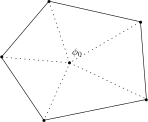
\includegraphics[width=0.8\textwidth]{../figures/lagrange_phi0.pdf}
        \caption{Lagrange element basis function at the center point}
    \end{figure}
\vspace{5pt}
\end{minipage}
\end{frame}

\begin{frame}
\frametitle{Numerical Examples}
Consider the following second-order elliptic equation:
$$
\left\{
\begin{aligned}
    -\Delta u + 2u & = f \quad \Omega \\
    u & = 0 \quad \partial\Omega
\end{aligned}
\right.
$$
where $\Omega = (0, 1)\times(0, 1)$, and the right-hand side and the exact solution are:
$$
u = \sin(\pi x)\sin(\pi y), \quad f = (2\pi^2+2)\sin(\pi x)\sin(\pi y).
$$

\begin{figure}[htbp]
\centering
\begin{minipage}[t]{0.49\linewidth}
\centering
\includegraphics[width=4cm]{../figures/convex.pdf}
\captionsetup{font={small}}
\caption{Convex polygon mesh $\mathcal T_0$}
\end{minipage}%
\begin{minipage}[t]{0.49\linewidth}
\centering
\includegraphics[width=4cm]{../figures/nonconvex.pdf}
\captionsetup{font={small}}
\caption{Non-convex polygon mesh $\mathcal T_1$}
\end{minipage}%
\centering
\end{figure}
\end{frame}

\begin{frame}
    \frametitle{Numerical Results: Convergence}
We choose $k = 1, 2, 5$ in both SFNCVEM and SFCVEM.
The numerical results of the SFNCVEM on meshes $\mathcal T_0$ and $\mathcal T_1$
as follow. We can see that $\|u - Q_h u_h\|_0=O(h^{k+1})$ and $\|\nabla u -
Q_{h}\nabla_h u_h\|_0=O(h^{k})$, 
\begin{figure}[htbp]
\centering
\begin{minipage}[t]{0.49\linewidth}
\centering
\includegraphics[width=5.5cm]{../figures/stabfree/ncvem_convex.pdf}
%\caption{Numberical result of example with $\mathcal T_0$.}
\end{minipage}%
\begin{minipage}[t]{0.49\linewidth}
\centering
\includegraphics[width=5.5cm]{../figures/stabfree/ncvem_nonconvex.pdf}
%\caption{[Numberical result of example with $\mathcal T_1$].}
\end{minipage}%
\centering
\caption{Errors $\|u - Q_h u_h\|_0$ and $\|\nabla u - Q_{h}\nabla_h u_h\|_0$
of nonconforming VEM on
$\mathcal T_0$(left) and $\mathcal T_1$(right) with $k=1, 2, 5$.}
\label{fig:rate1}
\end{figure}


\end{frame}

\begin{frame}
    \frametitle{Numerical Results: Convergence}
And the numerical results of the SFCVEM are presented as follow. 
Again $\|u - Q_h u_h\|_0=O(h^{k+1})$ and $\|\nabla u - Q_{h}\nabla
u_h\|_0=O(h^{k})$. 

\begin{figure}[htbp]
\centering
\begin{minipage}[t]{0.49\linewidth}
\centering
\includegraphics[width=5.5cm]{../figures/stabfree/cvem_convex.pdf}
%\caption{Numberical result of example with $\mathcal T_0$.}
\end{minipage}%
\begin{minipage}[t]{0.49\linewidth}
\centering
\includegraphics[width=5.5cm]{../figures/stabfree/cvem_nonconvex.pdf}
%\caption{[Numberical result of example with $\mathcal T_1$].}
\end{minipage}%
\centering
\caption{Errors $\|u - Q_h u_h\|_0$ and $\|\nabla u - Q_{h}\nabla u_h\|_0$
of conforming VEM on $\mathcal T_0$(left) and
$\mathcal T_1$(right) with $k=1, 2, 5$.}
\label{fig:rate2}
\end{figure}

\end{frame}

\begin{frame}
    \frametitle{Numerical Results: Condition Numbers}
We construct three different hexagons shown as follow, and calculate the
eigenvalues of local stiffness matrices with $k=3$ for four virtual element
methods. 
% \begin{figure}[htbp]
% \centering
% \subfigure{\includegraphics[width=1.4in]{./figures/hexagon0.pdf}}
%     % \caption{Type I:5 tetrahedra}
% %%
% \subfigure{\includegraphics[width=1.4in]{./figures/hexagon1.pdf}}
%      %\caption{Type II: 24 tetrahedra}
% %%
% \subfigure{\includegraphics[width=1.2in]{./figures/hexagon2.pdf}}
%      %\caption{Trirectangular tetrahedron}
% %%
% \caption{The regular hexagon(Left), the quasi-regular hexagon generated by regular
%     hexagon with a small perturbation (Middle), 
% and the square with two hanging nodes (Right)}
%   \label{fig:hexagon0} %% label for entire figure
% \end{figure}
\begin{figure}[htbp]
\centering
\begin{subfigure}[t]{0.3\linewidth}
    \centering
    \includegraphics[width=1in]{../figures/stabfree/hexagon0.pdf}
    \caption{Regular hexagon.}
    \label{fig:hexagon0}
\end{subfigure}%
\hspace{0.5cm} % 控制子图之间的水平间距
\begin{subfigure}[t]{0.3\linewidth}
    \centering
    \includegraphics[width=1in]{../figures/stabfree/hexagon1.pdf}
    \caption{Quasi-regular hexagon generated by regular hexagon with a small perturbation.}
    \label{fig:hexagon1}
\end{subfigure}%
\hspace{0.5cm} % 控制子图之间的水平间距
\begin{subfigure}[t]{0.3\linewidth}
    \centering
    \includegraphics[width=0.9in]{../figures/stabfree/hexagon2.pdf}
    \caption{Square with two hanging nodes.}
    \label{fig:hexagon2}
\end{subfigure}
\caption{The regular hexagon (Left), the quasi-regular hexagon generated by regular hexagon with a small perturbation (Middle), and the square with two hanging nodes (Right).}
\label{fig:all}
\end{figure}
\end{frame}

\begin{frame}
    \frametitle{Numerical Results: Condition Numbers}
We also present the minimum
non-zero eigenvalue, the maximum eigenvalue and the condition number for the
local stiffness matrix on different hexagons, from
which we can see that these quantities are comparable for four virtual element
methods.
\only<1>{
\begin{table}[htbp]
\centering
\caption{Comparison of eigenvalues and condition numbers on the regular hexagon.}
\begin{tabular}{c|ccc}
\hline
\textbf{方法} & \textbf{最大特征值} & \textbf{最小特征值} & \textbf{条件数} \\ \hline
NCVEM & 975.5693189 & 0.309674737 & 3150.303211 \\ \hline
CVEM & 1012.488116 & 0.297206358 & 3406.683909 \\ \hline
SFNCVEM & 992.5956147 & 0.318932029 & 3112.248147 \\ \hline
SFCVEM & 1011.173331 & 0.298509692 & 3387.405362 \\
\hline
\end{tabular}
\end{table}
}
\only<2>{
\begin{table}[htbp]
\centering
\caption{Comparison of eigenvalues and condition numbers on the quasi-regular hexagon.}
\begin{tabular}{c|ccc}
\hline
\textbf{方法} & \textbf{最大特征值} & \textbf{最小特征值} & \textbf{条件数} \\ \hline
NCVEM   & 935.2883848 & 0.279027715 & 3351.955143 \\ \hline
CVEM    & 1014.672395 & 0.257370621 & 3942.456177 \\ \hline
SFNCVEM & 997.4831245 & 0.282126359 & 3535.589964 \\ \hline
SFCVEM  & 1047.876056 & 0.258970708 &
4046.311124 \\
\hline
\end{tabular}
\end{table}
}
\only<3>{
\begin{table}[htbp]
\centering
\caption{Comparison of eigenvalues and condition numbers on the square with two hanging nodes.}
\begin{tabular}{c|ccc}
\hline
\textbf{方法} & \textbf{最大特征值} & \textbf{最小特征值} & \textbf{条件数} \\ \hline
 NCVEM   & 941.8571938&	0.21069027	&4470.340249 \\ \hline
 CVEM    & 1046.755495&	0.200435123	&5222.4155 \\ \hline
 SFNCVEM & 986.5963357&	0.212761106	&4637.108513 \\ \hline
 SFCVEM  & 1061.651989&	0.202074633	&5253.761808 \\
\hline
\end{tabular}
\end{table}
}
\end{frame}

\begin{frame}
\frametitle{Numerical Results: Computational Time}

We conducted experiments on convex polygonal meshes. The following table shows
that the assembly times for NCVEM, CVEM, and SFNCVEM are similar. However, due
to the need for SFCVEM to project onto a higher-order polynomial space, its
computational time is longer.
\only<1>{
\begin{table}[htbp]
\centering
\caption{Time taken to assemble the stiffness matrix for four VEM methods under different $k$ values ($h = 0.2$).}
\begin{tabular}{c|cccc}
\hline
\textbf{k} & \textbf{2} & \textbf{4} & \textbf{8} & \textbf{10} \\ \hline
SFCVEM & 0.053684235 & 0.144996881 & 1.468627453 & 2.603836536 \\ \hline
SFNCVEM & 0.022516727 & 0.065697193 & 0.806378841 & 1.554260015 \\ \hline
CVEM & 0.021185875 & 0.059809923 & 0.600241184 & 1.160929918 \\ \hline
NCVEM & 0.0213027 & 0.061014891 & 0.596506596 & 1.129639149 \\
\hline
\end{tabular}
\end{table}
}
\only<2>{
\begin{table}[htbp]
\centering
\caption{Time taken to assemble the stiffness matrix for four VEM methods under different $h$ values, with $k=5$.}
\begin{tabular}{c|cccc}
\hline
\textbf{h} & \textbf{1} & \textbf{0.25} & \textbf{0.0625} & \textbf{0.03125} \\ \hline
SFCVEM & 0.039689541 & 0.199015379 & 1.74412179 & 4.75462532 \\ \hline
SFNCVEM & 0.018287182 & 0.100006819 & 0.81251812 & 2.465409517 \\ \hline
CVEM & 0.018686771 & 0.087426662 & 0.781031132 & 1.983617783 \\ \hline
NCVEM & 0.018309593 & 0.096345425 & 0.767129898 & 2.159288645 \\
\hline
\end{tabular}
\end{table}
}
\end{frame}

%\section{时谐 Maxwell 方程的虚单元方法}
%\begin{frame}
%    \frametitle{时谐 Maxwell 方程界面问题}
%\begin{minipage}[b]{0.6\linewidth}
%    考虑如下时谐 Maxwell 方程:
%    $$
%    \left\{
%    \begin{aligned}
%        \mathbf{rot} \alpha \mathrm{rot} \boldsymbol{u} - \beta \boldsymbol{u} & = \boldsymbol{f} \quad
%        \Omega\\
%        u\times \mathbf{n} & = 0 \quad \partial\Omega
%    \end{aligned}
%    \right.
%    $$
%    其中 $\alpha > 0, \beta > 0$ 是分片常数:
%    $$
%    \alpha = \left\{
%    \begin{aligned}
%        \alpha_1 \quad & \text{in } \Omega^+,\\
%        \alpha_2 \quad & \text{in } \Omega^-,
%    \end{aligned}
%\right.\quad
%\beta = \left\{
%\begin{aligned}
%    \beta_1 \quad & \text{in } \Omega^+,\\
%    \beta_2 \quad & \text{in } \Omega^-,
%\end{aligned}
%\right.
%    $$
%    界面条件为:
%$$
%\begin{aligned}
%[\mathbf{u}\cdot\mathbf{t}]_{\Gamma} :=
%(\mathbf{u}^+\cdot\mathbf{t}-\mathbf{u}^-\cdot\mathbf{t})|_{\Gamma} = 0\\
%[\alpha \rot \mathbf{u}]_{\Gamma} := (\alpha \rot \mathbf{u}^+
%- \alpha \rot \mathbf{u}^-)|_{\Gamma} = 0.
%\end{aligned}
%$$
%\end{minipage}
%\hfill
%\begin{minipage}[b]{0.38\linewidth}
%    \centering
%    \begin{figure}[htpb]
%        \centering
%        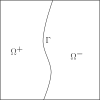
\includegraphics[width=0.8\textwidth]{../figures/interface_prob.pdf}
%        \caption{界面问题求解区域.}
%    \end{figure}
%\end{minipage}
%\end{frame}
%
%\begin{frame}
%  \frametitle{数值结果}
%  \begin{minipage}[b]{0.6\linewidth}
%    Set the domain and the interface geometry:
%    $$
%    \Omega = (-1, 1)\times(-1, 1), \quad \Omega^- = \{(x, y) : x^2+y^2 <
%\left(\frac{\pi}{5}\right)^2\},\quad \Omega^+ = \Omega - \Omega^-,
%    $$
%    Consider the parameters $\alpha|_{\Omega^-} = \beta|_{\Omega^-} = 1, 
%    \alpha|_{\Omega^+} = \beta|_{\Omega^+} = 10$, and the exact solution:
%    \small{
%    $$
%    {u} = \left\{
%        \begin{aligned}
%        & - k_0(r_0^2 - x^2 - y^2)
%        \begin{pmatrix}
%        y\\
%        x
%        \end{pmatrix} \quad& \Omega^-, \\
%        &-\frac{1}{10}
%        k_1(r_0^2 - x^2 - y^2)(r_1^2 - x^2 - y^2)
%        \begin{pmatrix}
%        y\\
%        x
%        \end{pmatrix}& \Omega^+, \\
%        \end{aligned} 
%    \right.
%    $$
%}
%    where $r_0 = \frac{\pi}{5}, r_1 = 1, k_1 = 20, k_0 = k_1(r_1^2-r_0^2).$
%\end{minipage}
%\hfill
%\begin{minipage}[b]{0.38\linewidth}
%    \centering
%    \begin{figure}[htpb]
%        \centering
%        \includegraphics[width=0.6\textwidth]{../figures/maxwell/convergence_test.pdf}
%        \caption{网格}
%    \end{figure}
%\end{minipage}
%
%\end{frame}
%
%\begin{frame}
%    \frametitle{数值结果}
%we can see that 
%$\|\mathbf{u} - \Pi_h \mathbf{u}_h\|_{0,\Omega} = O(h), \|\rot \mathbf{u} -
%\rot\mathbf{u}_h\|_{0,\Omega} = O(h)$ 
%which is clearly optimal.
%\begin{table}[!htp] 
%\centering
%\caption{Errors $||\mathbf{u} - \Pi_h \mathbf{u}_h||_{0,\Omega}$ and $||\rot
%\mathbf{u} - \rot \mathbf{u}_h||_{0,\Omega}$ }
%\label{tab:exm0}
%\begin{tabular}[c]{|c|c|c|c|c|c|c|}\hline
%$h$ & $1/8$ & $1/16$ & $1/32$ & $1/64$ 
%\\\hline
%$\|\mathbf{u} - \Pi_h{\mathbf{u}}_h \|_{0,\Omega}$ & 4.798e-01 & 2.192e-01 & 1.007e-01 & 4.761e-02 
%\\\hline
%Order & -- & 1.13 & 1.12 & 1.08 
%\\\hline
%$ \| \rot \mathbf{u} - \rot \mathbf{u}_h\|_{0,\Omega}$ & 1.155e+00 & 5.722e-01 & 2.726e-01 & 1.366e-01 
%\\\hline
%Order & -- & 1.01 & 1.07 & 1. 
%\\\hline
%\end{tabular}
%\end{table} 
%\end{frame}

\section{}

\section{Virtual Element Method for Moving Interface Problems}
\begin{frame}
    \frametitle{Parabolic Equation with Moving Interface}
\begin{minipage}[b]{0.6\linewidth}
\small{
We consider the following parabolic equation:
$$
\begin{aligned}
    \partial_t u - \nabla \cdot (\beta \nabla u) & = f, \quad \text{in} \quad \Omega \times (0, T)\\
    u & = 0, \quad \text{on} \quad \partial \Omega \times (0, T)\\
    u & = u_0, \quad \text{in} \quad \Omega \times \{0\}
\end{aligned}
$$
The coefficient $\beta$ is a piecewise constant function in $\Omega$:
$$
\beta(t) = 
\begin{cases}
    \beta^+(t), & \text{in} \quad \Omega^+(t)\\
    \beta^-(t), & \text{in} \quad \Omega^-(t)
\end{cases}
$$
The function $u$ satisfies the jump condition
on the interface $\Gamma(t)$:
$$
\begin{aligned}
    [u]|_{\Gamma(t)} = u^+|_{\Gamma(t)} - u^-|_{\Gamma(t)} = 0, \quad t\in (0,
    T)\\
[\beta \frac{\partial u}{\partial \boldsymbol{n}}]|_{\Gamma(t)} =
\beta^+\frac{\partial u^+}{\partial \boldsymbol{n}}|_{\Gamma(t)}
-
\beta^-\frac{\partial u^-}{\partial \boldsymbol{n}}|_{\Gamma(t)} = 0, \quad t\in (0, T)
\end{aligned}
$$
}
\end{minipage}
\hfill
\begin{minipage}[b]{0.38\linewidth}
\centering
\begin{figure}[htpb]
    \centering
    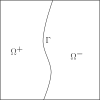
\includegraphics[width=0.8\textwidth]{../figures/interface_prob.pdf}
    \caption{The domain for solving the interface problem.}
\end{figure}
\vspace{25pt}
\end{minipage}

\end{frame}

\begin{frame}
\frametitle{FEM for Parabolic Equation with Moving Interface}
The Weak form of the parabolic equation is: Find $u \in H^1_0(\Omega)$
such that 
$$
(\partial_t u, v) + a(u, v) = (f, v), \quad \forall v \in H^1_0(\Omega)
$$
where 
$$
a(u, v) = \int_{\Omega} \beta \nabla u \cdot \nabla v \mathrm{d}x 
$$
When using the finite element method, the following issues may arise:
\begin{itemize}
    \item Mesh regeneration is required when the interface moves.
    \item Matrix reassembly is needed after mesh updates.
    \item The solution must be interpolated onto the new mesh after each update.
\end{itemize}
\end{frame}

\begin{frame}
    \frametitle{Mesh Generation}
\begin{figure}[htbp]
\begin{subfigure}[t]{0.49\linewidth}
    \centering
    \includegraphics[width=1.2in]{../figures/movingmaxwell/interface_half_cricle.pdf}
\end{subfigure}
\begin{subfigure}[t]{0.49\linewidth}
    \centering
    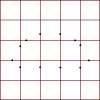
\includegraphics[width=1.2in]{../figures/movingmaxwell/cut_point.pdf}
\end{subfigure}
\end{figure}

\begin{figure}[htbp]
\begin{subfigure}[t]{0.49\linewidth}
    \centering
    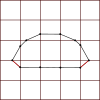
\includegraphics[width=1.2in]{../figures/movingmaxwell/cut_mesh_0.pdf}
\end{subfigure}
\begin{subfigure}[t]{0.49\linewidth}
    \centering
    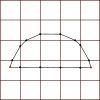
\includegraphics[width=1.2in]{../figures/movingmaxwell/cut_mesh_1.pdf}
\end{subfigure}
\end{figure}

\end{frame}

\begin{frame}
    \frametitle{Spatial Discretization}
Let $\mathcal{T}_h^b$ be the background mesh of $\Omega$, 
$\mathcal{T}_h^t$ is the mesh of $\Omega^{\pm}$ generated
by the algorithm above with interface $\Gamma^t$ 
and $V_h^t$ is the linear $H^1$ conforming virtual element space on
$\mathcal{T}_h^t$:
$$
V_K^t = \{v_h \in H^1(K): \Delta v_h = 0, v_h|_{\partial K} \in
    \mathbb{P}_1(K)\}
$$
The VEM is to find $u_h \in V_h^t$ statifies:
$$
(\partial_t u_h, \Pi_hv_h) + a_h(u_h, v_h) = 
(f, \Pi_hv_h), \quad \forall
v_h \in V_h^t
$$
where
$$
\begin{aligned}
    a_h(u_h, v_h) & := \sum_{K\in \mathcal{T}_h^t} a_K(u_h, v_h)\\
    a_K(u_h, v_h) & := (\beta\nabla \Pi_K u_h, \nabla \Pi_K v_h)_{K}
+ S_K( (I-\Pi_K) u_h, (I-\Pi_k)v_h)
\end{aligned}
$$
\end{frame}

\begin{frame}
    \frametitle{Time Discretization}
The time interval $[0, T]$ is divided into $N$ subintervals with the step size 
$\tau = T/N$, let $t^n = n\tau, n = 0, 1, \dots, N$. 
Define the backward difference operator:
$$
\delta_t u_h^n := \frac{\Pi_h^{n}u_h^n - \Pi_h^{n-1} u_h^{n-1}}{\tau}
$$
% 其中使用 $\Pi_h u_h^{n-1}$ 是为了可计算
Then replace the time derivative in VEM with the backward difference operator,
we obtain the following discrete problem: Find $u_h^n \in V_h^n$ statifies:
$$
(\delta_t u_h^n, \Pi_h^n v_h) + a_h(u_h^n, v_h) = (f^n,\Pi_h^n v_h)
\quad \forall v_h \in V_h^n
$$
rearrange the terms of equation above, we have: 
$$
\frac{1}{\tau}( \Pi_h^n u_h^n,\Pi_h^n v_h) + a_h(u_h^n, v_h) = 
(f^n, \Pi_h^n v_h) + \frac{1}{\tau}(\Pi_h^{n-1} u_h^{n-1},\Pi_h^n v_h)
\quad \forall v_h \in V_h^n
$$
\end{frame}

\begin{frame}
    \frametitle{The term $(\Pi_h^{n-1} u_h^{n-1},\Pi_h^n v_h)$}
The function $\Pi_h^{n-1} u^{n-1}_h$ 
in the term $\frac{1}{\tau}( \Pi_h^{n-1} u_h^{n-1}, \Pi_h^n v_h)$ 
is defined on the mesh $\mathcal{T}_h^{n-1}$, but $v_h$ is defined on the
mesh $\mathcal{T}_h^n$, so that the term 
$\frac{1}{\tau}( \Pi_h^{n-1} u_h^{n-1}, \Pi_h^n v_h)$
can't be computed directly. 
\begin{itemize}
    \item The function $\Pi_h u_h^{n-1}$ is a polynormial function on the
        $K_1^{n-1}$ or $K_2^{n-1}$. 
    \item The function $\Pi_h v_h$ is a polynormial function on the $K_1^n$ and
        $K_2^n$.
\end{itemize}

\begin{figure}[h]
    \centering
    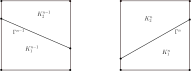
\includegraphics[width=2.8in]{../figures/movingmaxwell/backcell_be_cuted.pdf}
    % \caption{Type I:5 tetrahedra}
    \caption{\small The cell in background mesh be cuted by the interface $\Gamma^{n-1}$(Left),
    $\Gamma^n$(Right)} 
     \label{fig:overlapmesh} %% label for first subfigure
\end{figure}

\end{frame}


\begin{frame}
    \frametitle{The Middle Mesh}
We introduce a middle mesh $\mathcal{T}_h^{n-1/2}$, which is
generated by cuting the quadrilateral $K$ with the interface $\Gamma^{n-1}\cup\Gamma^n$.
$$
\begin{aligned}
    (\Pi_h u_h^{n-1}, \Pi_h v_h)_K = 
    &
    (\Pi_{K_1^{n-1}}u_h^{n-1}, \Pi_{K_1^{n}}v_h)_{K_1^{n-1/2}} 
    +
    (\Pi_{K_1^{n-1}}u_h^{n-1}, \Pi_{K_2^{n}}v_h)_{K_2^{n-1/2}}\\ 
    & +
    (\Pi_{K_2^{n-1}}u_h^{n-1}, \Pi_{K_2^{n}}v_h)_{K_3^{n-1/2}} 
    +
    (\Pi_{K_2^{n-1}}u_h^{n-1}, \Pi_{K_1^{n}}v_h)_{K_4^{n-1/2}} 
\end{aligned}
$$

\begin{figure}[h]
    \centering
    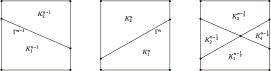
\includegraphics[width=4in]{../figures/movingmaxwell/overlap_interface.pdf}
    % \caption{Type I:5 tetrahedra}
    \caption{\small The cell in background mesh be cuted by the interface $\Gamma^{n-1}$(Left),
    $\Gamma^n$(Middle) and $\Gamma^{n-1} \cup \Gamma^n$(Right)}
     \label{fig:overlapmesh} %% label for first subfigure
\end{figure}
\end{frame}

\begin{frame}
    \frametitle{The Middle Mesh}
For the general
case, Similarlly, we cut the background mesh with the interface
$\Gamma^{n-1}\cup\Gamma^n$, 
then we can use the following formula to compute the term 
$(\Pi_h u_h^{n-1}, \Pi_h v_h)$:
$$
(\Pi_h u_h^{n-1}, \Pi_h v_h) = \sum_{K\in \mathcal{T}_h^{n-1/2}}
(\Pi_{K^{n-1}}u_h^{n-1}, \Pi_{K^n}v_h)_{K}
$$
where $K^{n}$ and $K^{n-1}$ is the parent element of $K$ on the mesh
$\mathcal{T}_h^n$ and $\mathcal{T}_h^{n-1}$ respectively,
\begin{figure}[h]
\centering
%%%%%
\begin{subfigure}{.3\textwidth}
    \centering
    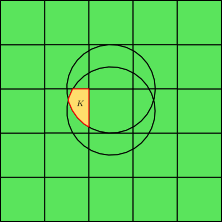
\includegraphics[width=1.05in]{../figures/movingmaxwell/meshncut.pdf}
\end{subfigure}
%%
\begin{subfigure}{.3\textwidth}
    \centering
    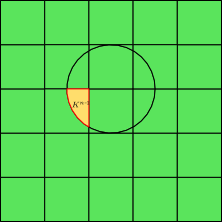
\includegraphics[width=1.05in]{../figures/movingmaxwell/meshn_1.pdf}
\end{subfigure}
%%
\begin{subfigure}{.3\textwidth}
    \centering
     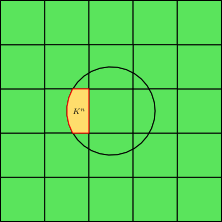
\includegraphics[width=1.05in]{../figures/movingmaxwell/meshn.pdf}
\end{subfigure}
\caption{The mesh $\mathcal{T}_h^{n-1/2}$(Left), $\mathcal{T}_h^{n-1}$(Middle)
    and $\mathcal{T}_h^{n}$(Right), where the element $K^{n}$ and $K^{n-1}$ is
the parent element of $K$.}
\end{figure}
\end{frame}

\begin{frame}
    \frametitle{Numerical Results : Convergence}
Consider a parabolic equation with a moving circle interface. 
The exact solution is:
\begin{equation}
  u(x,y,t) = \left\{ 
    \begin{matrix}
        \frac{r^3(x, y, t)}{\beta_0}, & \text{if } r(x, y, t) < R,\\
        \frac{r^3(x, y, t)}{\beta_1} + (\frac{1}{\beta_0} - \frac{1}{\beta_1})R^3, & \text{otherwise}.
    \end{matrix}
    \right.
\end{equation}
where $r(x, y, t) = \sqrt{(x-0.5)^2 + (y-0.7+0.2t)^2}$, $\beta_0 = 1$ and
$\beta_1 = 100$.

% t=0 时刻和 t=1 时刻的界面
\begin{figure}[H]
    \begin{minipage}[t]{0.49\linewidth}
        \centering
        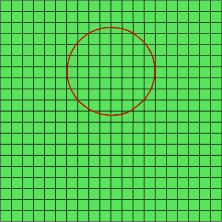
\includegraphics[width=0.5\textwidth]{../figures/movingmaxwell/circle_interface_0.pdf}
    \end{minipage}
    \begin{minipage}[t]{0.49\linewidth}
        \centering
        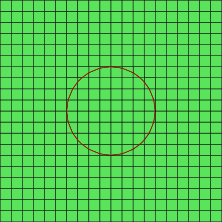
\includegraphics[width=0.5\textwidth]{../figures/movingmaxwell/circle_interface_1.pdf}
    \end{minipage}
    \caption{The domain and circle interface at $t=0$ (left) and $t=1$ (right).}
\end{figure}
\end{frame}

\begin{frame}{Convergence and Computational Efficiency}
\frametitle{Convergence Analysis}
\small{
\begin{table}[h]
\centering
\caption{Convergence rates for different error norms.}
\begin{tabular}{|c|c|c|c|c|c|}
\hline
$h$ & 0.05 & 0.025 & 0.0125 & 0.00625 & 0.003125 \\
\hline
$|u-u_h|{\Omega}$ & 1.76E-05 & 5.30E-06 & 1.41E-06 & 3.63E-07 &
9.54E-08 \\
\hline
$\mathrm{order}$ & - & 1.73 & 1.90 & 1.96 & 1.93 \\
\hline
$|u-u_h|{1, \Omega}$ & 0.0019113 & 0.0009444 & 0.0004515 &
0.000226708 & 0.0001122 \\
\hline
$\mathrm{order}$ & - & 1.01 & 1.06 & 0.99 & 1.01 \\
\hline
$|u-u_h|_{\infty,\Omega}$ & 0.0001298 & 3.58E-05 & 8.25E-06 &
2.45E-06 & 5.45E-07 \\
\hline
$\mathrm{order}$ & - & 1.86 & 2.11 & 1.75 & 2.16 \\
\hline
\end{tabular}
\end{table}

%One advantage of our algorithm is that it only requires assembling matrices on interface elements. The table below compares the time taken to assemble all matrices versus only interface matrices on different grid sizes. Assembling interface matrices is significantly faster.

\begin{table}[h]
\centering
\caption{Comparison of computational times.}
\begin{tabular}{|c|c|c|c|c|c|c|}
\hline
$h$ & 0.1 & 0.05 & 0.025 & 0.0125 & 0.00625 & 0.003125 \\
\hline
\makecell{Time to Assemble \\ All Matrices (s)} & 0.079 & 0.31 & 0.88 & 2.99 & 12.38 & 46.27 \\
\hline
\makecell{Time to Assemble \\ Interface Matrices (s)} & 0.031 & 0.14 & 0.25 & 0.73 & 1.87 & 6.27 \\
\hline
\end{tabular}
\end{table}
}
\end{frame}

\begin{frame}
    \frametitle{Eddy Current Equation}
Consider the following eddy current equation for the 
vector potential $\boldsymbol{A}$:
$$
\sigma\partial_t \boldsymbol{A}+\nabla\times(\mu^{-1}\nabla\times \boldsymbol{A}) 
- \sigma\boldsymbol{v}\times (\nabla\times\boldsymbol{A}) = 
\nabla\times \boldsymbol{M} + \boldsymbol{J}_s
$$
where $\sigma$ is the conductivity, $\mu$ is the magnetic permeability, they are
piecewise constant functions. $\boldsymbol{A}$ statify the interface condition.
$$
[\![(\mu^{-1}\nabla\times \boldsymbol{A})\times \boldsymbol{n}]\!]|_{\Gamma} = 
[\![\boldsymbol{M}\times \boldsymbol{n}]\!]|_{\Gamma}
$$
\begin{figure}[htpb]
    \centering
    \includegraphics[width=0.3\textwidth]{../figures/movingmaxwell/eddycurrent_domain.pdf}
    \caption{The domain for solving the eddy current problem.}
\end{figure}
\end{frame}

\begin{frame}
  \frametitle{Eddy Current Equation in Cylindrical Coordinates}
  \begin{minipage}[b]{0.56\linewidth}
    Assume the computational domain is axisymmetric, and:
    $$
    \boldsymbol{J}_s = J_s \bse_{\theta}, \quad \boldsymbol{A} = A \bse_{\theta}, \quad \boldsymbol{M} = M_r \bse_r + M_z \bse_z
    $$
    with all variables independent of the $\theta$ direction. The 3D eddy current equation can then be reduced to a 2D form:
    $$
    \begin{aligned}
    \sigma \partial_t A \bse_{\theta}& + \nabla \times \left( \mu^{-1} \nabla
\times A \bse_{\theta} \right) \\
    & - \sigma \boldsymbol{v} \times \left( \nabla \times A \bse_{\theta}
    \right) = \nabla \times \boldsymbol{M} + J_s \bse_{\theta}
    \end{aligned}
    $$
    \vspace{10pt}
  \end{minipage}
  \hfill
  \begin{minipage}[b]{0.38\linewidth}
    \centering
    \begin{figure}[htpb]
      \centering
      \includegraphics[width=0.5\textwidth]{../figures/movingmaxwell/rzplane.pdf}
      \caption{The $rz$ plane of the cylinder.}
    \end{figure}
  \end{minipage}
\end{frame}

\begin{frame}
    \frametitle{Magnet Falling in Copper Tube}
\begin{minipage}[b]{0.6\linewidth}
%As the magnet falls through the copper tube, eddy currents are generated, converting mechanical energy into heat. According to Lenz's Law, these eddy currents create a magnetic field that opposes the magnet's motion. As a result, the magnet experiences both gravitational and magnetic forces, eventually reaching a terminal velocity where the speed no longer increases.
\textbf{Copper Tube Data:}
\begin{itemize}
    \item Inner Diameter: 7.85 mm
    \item Wall Thickness: 1.9 mm
    \item Length: 1.7 m
    \item Conductivity: \( 5.998 \times 10^7 \, \text{S/m} \)
    \item Permeability: \( 4\pi \times 10^{-7} \, \text{H/m} \)
\end{itemize}

\textbf{Magnet Data:}
\begin{itemize}
    \item Radius: 6.35 mm
    \item Height: 6.35 mm
    \item Conductivity: \( 7.14 \times 10^5 \, \text{S/m} \)
    \item Permeability: \( 4\pi \times 10^{-7} \, \text{H/m} \)
    \item Magnetization: \( \frac{1.41}{4\pi \times 10^{-7}} \)
\end{itemize}
\vspace{10pt}
\end{minipage}
\hfill
\begin{minipage}[b]{0.38\linewidth}
    \centering
    \begin{figure}[htpb]
        \centering
        \includegraphics[width=0.4\textwidth]{../figures/movingmaxwell/magnet_falling.pdf}
        \caption{The magnet falling in the copper tube.}
    \end{figure}
\end{minipage}

\end{frame}

\begin{frame}
    \frametitle{Magnet Falling in Copper Tube}
    \begin{figure}[htpb]
    \centering
    \begin{subfigure}[t]{0.49\linewidth}
        \centering
        \includegraphics[width=0.4\textwidth]{../figures/movingmaxwell/J_magnet.jpg}
    \end{subfigure}
    \begin{subfigure}[t]{0.49\linewidth}
        \centering
        \includegraphics[width=0.8\textwidth]{../figures/movingmaxwell/v.png}
    \end{subfigure}
    \caption{The eddy current density at $t=0.03s$ (left) and the velocity of the
    magnet (right).}
\end{figure}
\end{frame}

\begin{frame}
    \frametitle{Electromagnetic Forming}
\begin{figure}[htpb]
    \centering
    \includegraphics[width=0.7\textwidth]{../figures/movingmaxwell/EMF.pdf}
    \caption{The Domain for Electromagnetic Forming.}
\end{figure}
\end{frame}

\begin{frame}
  \frametitle{Electromagnetic Forming}
  \begin{figure}[htpb]
    \centering
    \begin{subfigure}[t]{0.49\linewidth}
        \centering
        \includegraphics[width=0.8\textwidth]{../figures/movingmaxwell/J10.png}
    \end{subfigure}
    \begin{subfigure}[t]{0.49\linewidth}
        \centering
        \includegraphics[width=0.8\textwidth]{../figures/movingmaxwell/v_plot.pdf}
    \end{subfigure}
    \caption{The eddy current density at $t=1e-5$ (left) and the velocity of the 
    workpiece (right).}
\end{figure}
\end{frame}



%\section{虚单元方法的实现}
%\subsection{网格}
%\begin{frame}
%    \frametitle{数组化的半边数据结构}
%    \begin{onlyenv}<1>
%
%    \begin{columns}
%       \column{0.4\textwidth}
%       \centering
%       \begin{figure}[htb]
%           \includegraphics[scale=0.3]{../figures/cell.png}
%         \caption{半边数据结构网格}
%       \end{figure}
%       \column{0.6\textwidth}
%       \vspace{1pt}
%       {\scriptsize
%       \begin{tabular}{cccc}
%           \hline
%           半边 & 邻接信息 & 半边 & 邻接信息\\
%           \hline
%           \hline
%           0 & [0, 0, 6, 2, 1] & 5 & [3, 2, 7, 8, 4]\\
%           1 & [1, 1, 3, 9, 0] & 6 & [3, 0, 4, 0, 7]\\
%           2 & [1, 0, 0, 4, 3] & 7 & [0, 2, 8, 5, 6]\\
%           3 & [2, 1, 9, 1, 2] & 8 & [2, 2, 5, 7, 9]\\
%           4 & [2, 0, 2, 6, 5] & 9 & [0, 1, 1, 3, 8]\\
%           \hline
%       \end{tabular}}
%       \captionof{table}{半边邻接信息}
%    \end{columns}
%    \begin{table}[htb]
%        \begin{minipage}[b]{.5\linewidth}
%            \centering
%            \begin{tabular}{cc}
%                \hline
%                起始半边 & [6, 9, 8]\\
%                \hline
%            \end{tabular}
%            \caption{单元起始半边}
%        \end{minipage}%
%        \begin{minipage}[b]{.5\linewidth}
%            \begin{tabular}{cc}
%                \hline
%                主半边 & [1, 3, 5, 7, 8]\\
%                \hline
%            \end{tabular}
%            \caption{主半边}
%        \end{minipage}
%    \end{table}
%    \end{onlyenv}
%\end{frame}
%
%\subsection{虚单元空间}
%\begin{frame}
%    \frametitle{缩放单项式空间}
%\begin{minipage}[b]{0.55\linewidth}
%For $\boldsymbol{\alpha} = (\alpha_0, \alpha_1) \in \mathcal{A}_k^2$, 
%we can define the scaling monomial on $K$ as follows:
%$$
%m_{\boldsymbol{\alpha}}(x, y) = \frac{(x - x_K)^{\alpha_0}(y -
%y_K)^{\alpha_1}}{h_K^{|\boldsymbol{\alpha}|}}
%$$
%where
%\begin{itemize}
%    \item $h_K$ denoting size of $K$. 
%    \item $\boldsymbol{x_K} = (x_K, y_K)$ is the barycenter of $K$.
%\end{itemize}
%$\boldsymbol{m_k} = [m_0, m_1, m_2, \cdots, m_{n_k-1}], $
%which forms a basis for the scalar space $\mathbb{P}_k(K)$.
%\end{minipage}
%\hfill
%\begin{minipage}[b]{0.4\linewidth}
%    \centering
%    \begin{figure}[htpb]
%        \centering
%        \includegraphics[width=0.8\textwidth]{../figures/polygon_K.png}
%        \caption{Barycenter of $K$.}
%    \end{figure}
%\end{minipage}
%\end{frame}
%
%\begin{frame}
%  \frametitle{缩放单项式求导}
%  \begin{itemize}
%      \item $\partial_x$ and $\partial_y$ is a linear map from $\mathbb{P}_k(K) \to
%          \mathbb{P}_k(K)$.
%          $$
%          \partial_x m_{ \boldsymbol \alpha} = 
%            \begin{cases}
%            \frac{1}{h_K}\alpha_0 m_{\boldsymbol \alpha-(1, 0)} \quad & \alpha_0 > 0\\
%            \quad 0 & \alpha_0 = 0
%            \end{cases}
%          $$
%          define a matrix $P^x, P^y$:
%          $$
%          P_{\boldsymbol{\alpha\beta}}^x =
%            \begin{cases}
%            \frac{1}{h_K}\alpha_0 \quad & \boldsymbol \beta = \boldsymbol \alpha - (1, 0)\\
%             0 & \mathrm{other}
%         \end{cases},
%            P^y_{ \boldsymbol{\alpha\beta}} =
%            \begin{cases}
%            \frac{1}{h_K}\alpha_1 \quad & \boldsymbol \beta = \boldsymbol \alpha - (0, 1)\\
%             0 & \mathrm{other}
%            \end{cases}
%          $$
%      \item the matrix representation of $\frac{\partial }{\partial
%          \boldsymbol{t}}$ and $\frac{\partial^2 }{\partial
%          \boldsymbol{t}\partial \boldsymbol{n}}$ is
%          $$
%          P^{\boldsymbol{t}} = t_0 P^x + t_1 P^y, \quad 
%          P^{\boldsymbol{t}\boldsymbol{n}}= P^{\boldsymbol{t}}P^{\boldsymbol{n}}
%          $$.
%  \end{itemize}
%
%
%\end{frame}
%
%\begin{frame}
%  \frametitle{缩放单项式的积分}
%缩放单项式积分计算简单,因为缩放单项式是齐次函数,而
%齐次函数在单元 $K$ 上的积分可以化简到单元边界上的积分。对于一个齐次函数 
%$f$,其满足:
%$$
%f(k \bsx) = k^q f(\bsx)
%$$
%令等式两边同是对 $k$ 求导,可得
%$$
%\nabla f(k \bsx)\cdot \bsx = q k^{q-1} f(\bsx)
%$$
%令 $k = 1$,可得
%$$
%f(\bsx) = \frac{1}{q} \nabla f(\bsx)\cdot \bsx
%$$
%那么:
%$$
%\int_K f(\bsx)d\bsx = \frac{1}{q} \int_{K}
%\nabla f(\bsx)\cdot \bsx d\bsx
%= -\frac{1}{q} \int_{K} f(\bsx)\mathrm{div}{\bsx}
%\mathrm{d}\bsx
%+ \frac{1}{q} \int_{\partial K} f(\bsx)\bsx\cdot
%\bsn\mathrm{d}s
%$$
%注意 $\mathrm{div}{\bsx} = n$,
%所以我们可以把积分化简到单元边界上的积分:
%$$
%\int_K f(\bsx)\mathrm{d}\bsx = \frac{1}{q+n} \int_{\partial K}
%f(\bsx)\bsx\cdot \bsn\mathrm{d}s
%$$
%\end{frame}
%
%\begin{frame}
%  \frametitle{缩放单项式的积分}
%上式对于任意 $n$ 维多面体 $K$,以及任意齐次函数 $f$
%都成立,对于边界是平面的多面体,
%边界上的积分还可以进一步化简,
%令 $\mathcal{F}$ 为 $K$ 的边界面集合,对于 $F\in \mathcal{F}$,找到一个点
%$\bsx_F$ 在 $F$ 所在平面上,那么 
%$(\boldsymbol{x-x}_F)\cdot \bsn_F = 0$,
%所以
%$$
%\int_{\partial K} f(\bsx)\bsx\cdot \bsn
%\mathrm{d}s = \sum_{F\in \mathcal{F}}
%\int_{F} f(\bsx)(\boldsymbol{x-x_F+x_F})\cdot \bsn_F
%\mathrm{d}s = \sum_{F\in \mathcal{F}}
%\int_{F} f(\bsx)\boldsymbol{x_F}\cdot \bsn_F
%\mathrm{d}s
%$$
%
%而缩放单项式 $m_{\boldsymbol{\alpha}}$
%是一个齐次函数:
%$$
%m_{\boldsymbol{\alpha}}(k\bsx) = k^{|\boldsymbol{\alpha}|}
%m_{\boldsymbol{\alpha}}(\bsx)
%$$
%所以其在单元上的积分可以化简到单元边界上的积分:
%$$
%\int_K m_{\boldsymbol{\alpha}}(\bsx)\mathrm{d}\bsx =
%\frac{1}{|\boldsymbol{\alpha}|+n} \int_{\partial K}
%m_{\boldsymbol{\alpha}}(\bsx)\bsx\cdot \bsn
%\mathrm{d}s
%$$
%\end{frame}
%
%\begin{frame}
%    \frametitle{缩放单项式的质量矩阵,刚度矩阵}
%$m_{\boldsymbol{\alpha}}m_{\boldsymbol{\beta}} =
%m_{\boldsymbol{\alpha+\beta}}$,所以缩放单项式的质量矩阵为
%$$
%\bsM^{K}_{\boldsymbol{\alpha\beta}} = \int_K
%m_{\boldsymbol{\alpha}}m_{\boldsymbol{\beta}}\mathrm{d}\bsx =
%\frac{1}{|\boldsymbol{\alpha}+\boldsymbol{\beta}|+n} \int_{\partial K}
%m_{\boldsymbol{\alpha}}m_{\boldsymbol{\beta}}\bsx\cdot \bsn
%\mathrm{d}s
%$$
%刚度矩阵为:
%$$
%\begin{aligned}
%\bsA^{K}_{\boldsymbol{\alpha\beta}} & = \int_K
%\nabla m_{\boldsymbol{\alpha}}\cdot \nabla
%m_{\boldsymbol{\beta}}\mathrm{d}\bsx\\
%& = 
%\sum_{i=0}^{n-1} \int_K \partial_{x_i} m_{\boldsymbol{\alpha}}
%\partial_{x_i} m_{\boldsymbol{\beta}}\mathrm{d}\bsx
%& = \sum_{i=0}^{n-1} P^{K, i}_{\boldsymbol{\alpha\gamma}}
%\int_K m_{\boldsymbol{\gamma}}m_{\boldsymbol{\delta}}\mathrm{d}\bsx
%P^{K, i}_{\boldsymbol{\beta\delta}}
%\end{aligned}
%$$
%即: $A^{K} = \sum_{i=0}^{n-1} \bsP^{K, i}
%\bsM^{K} (\bsP^{K, i})^T = \frac{1}{h_K^2}
%\sum_{i=0}^{n-1} \bsP^{i} \bsM (\bsP^{i})^T$。
%同理,对于任意 $m>0$, 定义:
%$$
%A^{K, m}_{\boldsymbol{\alpha\beta}} = \int_K \nabla^m m_{\boldsymbol{\alpha}}
%\cdot \nabla^m m_{\boldsymbol{\beta}}\mathrm{d}\bsx
%$$
%\end{frame}
%
\end{CJK}
\end{document}




